% ======================================================================
% Paper 3 — Ledgers: Admissible Dynamics, Entropy, and the Arrow of Time
% v1.0: Initial draft
% v1.1-PLEC (2026-04-17): Surface-level PLEC propagation. No theorem
%   statements or proofs changed. Abstract and §1 gain PLEC framing and
%   the subordination sentence. T_kappa upper-bound attribution corrected
%   from "A1 minimality" to A2 (the argmin component of PLEC).
%   Appendix B assumption inventory expanded to include A2 as the fourth
%   PLEC component, matching Papers 1 v4.0-PLEC and 2 v5.3-PLEC.
% v3.0 (2026-04-17): Scope expansion. Sweeps in content from Early
%   Papers 3/34/35/36/39 and the 2026-04 partition-function/saturation-
%   exactness investigations. New sections:
%     (a) Ledger-accounting principle paragraph in §5 Entropy:
%         entropy as multiplicity count, robust under cost-landscape
%         corrections (from saturation-exactness report).
%     (b) Part II closing section "Geometric Carrying Capacity" —
%         Admissibility Carrying Capacity (ACC) extends enforcement
%         cost to geometric interfaces; 1/2 × 1/2 horizon-entropy
%         bookkeeping factors; unification of thermodynamic,
%         entanglement, and horizon entropy as three views of
%         interface-capacity saturation.
%     (c) Two new Arrow-of-Time subsections: macroscopic arrow from
%         loss of global admissible coordination; low-entropy initial
%         state reframed as restricted phase space (not improbable
%         order), rebutting the typicality argument.
%     (d) Part III section "Cosmogenesis and Staged Relaxation":
%         constraint functional Phi_c = ln(d_field / d_admissible);
%         overconstrained initial regime; staged constraint relaxation
%         → scale-dependent imprints; trapped-surface threshold;
%         horizon enforceability preview (Paper 39 / Paper 6).
%   Minor v1.2 coderef completions folded in: T_deSitter_entropy,
%   L_crossing_entropy, L_Fisher_entropy_budget added to theorem index;
%   Part I T_tensor, L_nc, L_loc coderefs marked explicitly. Two new
%   falsifiers F4 (GW ringdown memory) and F5 (structured primordial
%   imprints) added. Appendix C updated.
% ======================================================================

\documentclass[11pt]{article}

\usepackage[T1]{fontenc}
\usepackage[utf8]{inputenc}
\usepackage[a4paper,margin=1in]{geometry}
\usepackage{setspace}
\usepackage{parskip}
\usepackage{enumitem}
\usepackage{booktabs}
\usepackage{array}
\usepackage{amsmath,amssymb,amsfonts}
\usepackage{mathtools}
\usepackage[most]{tcolorbox}
\usepackage{tikz}
\usepackage{graphicx}
\usetikzlibrary{positioning,arrows.meta}
\usepackage{titlesec}
\usepackage{fancyhdr}

\titleformat{\section}{\Large\bfseries}{\thesection.}{0.5em}{}
\titleformat{\subsection}{\large\bfseries}{\thesubsection}{0.5em}{}
\titleformat{\subsubsection}{\normalsize\bfseries}{\thesubsubsection}{0.5em}{}

\pagestyle{fancy}
\fancyhf{}
\fancyhead[L]{\small\itshape Paper 3: Ledgers}
\fancyhead[R]{\small\itshape E.\,Brooke}
\fancyfoot[C]{\thepage}
\renewcommand{\headrulewidth}{0.4pt}

\usepackage[colorlinks=true,linkcolor=black,citecolor=black,urlcolor=black]{hyperref}

\tcbuselibrary{skins,breakable}

\tcbset{
    apfbox/.style={
        enhanced,
        colback=black!3,
        frame hidden,
        borderline={0.5pt}{0pt}{black},
        arc=0pt,
        left=8pt, right=8pt, top=8pt, bottom=8pt,
        fonttitle=\bfseries\color{black},
        coltitle=black,
        detach title,
        before upper={\tcbtitle\par\smallskip},
        before skip=14pt,
        after skip=14pt,
        grow to left by=-8pt,
        grow to right by=-8pt,
        sharp corners,
        breakable,
    }
}

\newenvironment{varlist}{\begin{itemize}[nosep,leftmargin=2em]}{\end{itemize}}
\newcommand{\coderef}[2]{\smallskip\noindent\textit{Code reference:} \texttt{#1} in \texttt{#2}.}
\newcommand{\SU}{\mathrm{SU}}
\newcommand{\U}{\mathrm{U}}
\newcommand{\epitag}[1]{\textbf{[#1]}}

\title{
  \textbf{Paper 3: Ledgers}\\
  \large Admissible Dynamics, Entropy, and the Arrow of Time\\
  \normalsize v3.0\\
  \normalsize E.\ S.\ Brooke\\
  Admissibility Physics --- March 2026 (v3.0 scope expansion: April 2026)
}
\author{}
\date{}

\setstretch{1.05}
\setlist[itemize]{itemsep=3pt,topsep=4pt}
\setlist[enumerate]{itemsep=3pt,topsep=4pt}

% ---- DAG style ----
\tikzset{
  dagbox/.style={draw, rounded corners=2pt, fill=black!5,
    font=\small, inner xsep=5pt, inner ysep=3pt,
    align=center, minimum width=1.7cm, text depth=1pt},
  dagsbox/.style={draw, rounded corners=2pt, fill=black!5,
    font=\footnotesize, inner xsep=4pt, inner ysep=2pt,
    align=center, text depth=1pt},
  dagarr/.style={-{Stealth[length=4pt,width=3.5pt]}, semithick},
}

\begin{document}
\maketitle

\begin{abstract}
\noindent
Paper~2: \emph{The Structure of Admissible Physics} established that the
correlation space has a unique architecture: a gauge group
$\SU(3)\times\SU(2)\times\U(1)$, a fermion content of 45~Weyl fermions in
three generations, and a capacity partition $42+19=61$ that fixes the
cosmological density fractions.  The space has rooms, and we can count them.
What it does not yet have is a direction.

This paper supplies the arrow.

We derive three results from the foundation of Paper~1, all following from
the four structurally necessary components of the \emph{Principle of Least
Enforcement Cost} (PLEC) -- A1 (finite enforcement capacity, upper bound),
MD (positive cost floor), A2 (argmin selection), BW (non-degeneracy) --
together with the tensor product structure established in Paper~1
($T_{\mathrm{tensor}}$):

\begin{enumerate}[nosep]
\item \textbf{Complete positivity as a theorem ($T_{\mathrm{CPTP}}$):}
  Admissibility-preserving evolution maps are exactly the completely positive,
  trace-preserving (CPTP) maps.  This closes the conditional result deferred
  from Paper~1, where ancilla-stability required analysis of how admissible
  maps compose under tensor products.  The Stinespring dilation~\cite{Stinespring1955}
  receives a direct enforcement interpretation: system and environment evolve unitarily
  with separate budgets, then the environment budget is traced out.

\item \textbf{Entropy as committed capacity ($T_{\mathrm{entropy}}$,
  $T_{\kappa}$):} The von Neumann entropy of a state equals the enforcement
  demand of its active correlations at the system interface.  The directed
  enforcement multiplier $\kappa=2$ is derived (not postulated) from
  irreversibility and locality.  The zeroth and first laws of thermodynamics
  follow as corollaries.

\item \textbf{The arrow of time from irreversibility ($L_{\mathrm{irr}}$,
  $T_{\mathrm{second\,law}}$):} Capacity committed to system-environment
  correlations cannot be recovered by any local operation.  This is not a
  boundary condition; it is forced by A1, $L_{\mathrm{nc}}$, and
  $L_{\mathrm{loc}}$.  The direction of non-decreasing entropy is the arrow
  of time.  $T$-violation of phase $\pi/4$ quantifies the asymmetry.
\end{enumerate}

These results sit inside the variational framework that Papers~1 and~2 now
present as the \emph{Principle of Least Enforcement Cost} (PLEC): reality as
the minimum-cost expression of distinction compatible with finite capacity,
with A1 (finite capacity; upper bound), MD (positive cost floor), A2 (argmin
selection), and BW (non-degeneracy) as its four structurally necessary
components.  Paper~3 introduces no new components; the results above are
downstream consequences of the same four.

A secondary result, derived from the capacity-counting structure of Paper~2,
identifies the Fisher information metric on the space of admissible states as
a direct consequence of the entropy functional, and shows that RG flow is
Fisher gradient descent.  Two distinct CP-violation mechanisms emerge from
the single irreversibility lemma $L_{\mathrm{irr}}$: holonomy phases (CKM)
and entropy-optimization phases (PMNS).

Paper~3 also serves as the entropy paper at cosmological scale.  Enforcement
cost is the quantum-interface face of a more general capacity concept---the
\emph{admissibility carrying capacity} (ACC) of a relational interface,
whether that interface is a bipartite quantum split, a causal horizon, or the
cosmological boundary.  Part~II closes with a geometric extension that
recovers horizon entropy (prefactor $1/4$) as a special case of the same
ledger accounting; Part~III extends the arrow of time to a macroscopic
regime where the arrow is identified with loss of global admissible
coordination, and closes with a structural treatment of cosmogenesis in which
low initial entropy is reframed as restricted admissible phase space and
cosmogenesis proceeds by staged constraint relaxation.

No new axioms are introduced.  All results trace to named check functions in
the codebase.  The paper is structured in three parts: Part~I (admissible
dynamics), Part~II (entropy, thermodynamics, and geometric carrying
capacity), and Part~III (time, cosmogenesis, information geometry, and CP
structure).
\end{abstract}

\tableofcontents
\newpage


% ======================================================================
\section{Introduction: the correlation space needs a direction}
\label{sec:intro}
% ======================================================================

Paper~1 and Paper~2 together built a static picture.  Paper~1 showed that
finite enforcement capacity forces a quantum operator algebra, a state space,
and a gauge symmetry.  Paper~2 showed that the only algebra compatible with
A1 is $\SU(3)\times\SU(2)\times\U(1)$ acting on the Standard Model fermion
content, and that the capacity budget partitions into 42~vacuum channels and
19~matter channels.  The correlation space $\mathcal{S}_{\mathrm{adm}}$ has
been mapped, measured, and classified.

But a map is not a movie.  The space as described so far has no preferred
direction, no thermodynamic interpretation, and no intrinsic notion of past
versus future.  Time appears as an external parameter.  Entropy is a
functional on states, but nothing has been said about how it changes, or why
it changes in a particular direction.

\begin{figure}[h]
\centering
\includegraphics[width=0.78\textwidth]{Fig_Admissible_States_Diagram.pdf}
\caption{\textbf{The geometry this paper makes dynamical.}  The upper bulb
is the admissible class $\mathcal{S}_{\mathrm{adm}}$ inherited from
Paper~2 --- a bounded region in correlation-capacity space, ``everything
allowed'' inside, ``not admissible'' on either flank.  The downward
arrow is the move this paper makes: \emph{time as a direction through the
volume}, generated not by an external parameter but by the irreversible
accumulation of locked correlations ($L_{\mathrm{irr}}$, Section~\ref{sec:arrow}).
Each cross-section of the volume at a given accumulated cost is an
\emph{entropy slice} (\S\ref{sec:entropy}, \S\ref{sec:gcc}): an interface
on which the remaining active capacity defines an entropy and on which
probability assignments become well-defined.  Entropy is the
\emph{area} of that slice, in the sense of the interface-area scaling
that yields $S_H = A/4$ in \S\ref{sec:gcc}, not a literal two-dimensional
surface.  At the narrow neck near the bottom, branching corresponds to
non-unique least-cost continuations (Type~II regime exit in Paper~6
\S7); the locking interface in the bottom-left icon is the
$L_{\mathrm{irr}}$ mechanism by which correlation pathways become
\emph{locally inaccessible} (capacity is committed at both sides of the
interface and no local observer can free it; this is the v6.8/v6.9
formulation of $L_{\mathrm{irr}}$, not the older ``infinite reverse cost''
formulation).  The downstream tubes are exclusive
correlation histories --- the record-locked sectors of Paper~5's $T9$.
Paper~3 builds this picture formally: \S2--3 derive admissibility-preserving
evolution as the CPTP maps; \S4--6 show that entropy on the slice equals
committed capacity; \S7 gets the second law from $L_{\mathrm{irr}}$; \S8
selects the orientation of the time arrow.  The diagram is the geometry
the rest of this paper makes dynamical.}
\label{fig:admissible-states}
\end{figure}

This paper shows that both the dynamics and the arrow arise from the same
source as everything else: the four-component variational structure that
Papers~1 and~2 call the \emph{Principle of Least Enforcement Cost} (PLEC),
of which A1 is the upper-bound component.

That source can be stated compactly.  PLEC -- reality as the minimum-cost
expression of distinction compatible with finite capacity -- packages
A1 (upper bound), MD (positive floor), A2 (argmin), and BW (non-degeneracy)
as four structurally necessary components of a single variational
principle.  PLEC is the canonical variational formulation of
the finite-enforceability framework; it does not replace the locked claim
that physical meaning is grounded in enforceable distinction.  In this
paper, ``A1'' continues to denote the finite-capacity component; the
argmin, floor, and non-degeneracy components (A2, MD, BW) enter where
selection and separation are at stake.

The argument has a natural structure.  Before we can ask how the correlation
space \emph{evolves}, we need to characterize which evolution maps are
admissibility-preserving.  That is Section~\ref{sec:cptp}: the answer is the
CPTP maps, as a theorem rather than a definition.  Once we know what
evolution looks like, we can ask what it does to entropy: Section~\ref{sec:entropy}
shows that entropy equals committed capacity, and derives the
directed-enforcement multiplier $\kappa=2$ from locality and irreversibility.
The zeroth and first laws of thermodynamics follow.

The second law requires a different argument, because it is not a statement
about what maps \emph{preserve} but about what the world \emph{does}.
Section~\ref{sec:secondlaw} derives it from $L_{\mathrm{irr}}$: the lemma
that cross-interface correlations commit capacity that no local observer can
recover.  Section~\ref{sec:arrow} shows that this lemma selects an
orientation on the single timelike direction forced by the Lorentzian
signature of spacetime (Paper~5), and that $T$-violation at phase $\pi/4$
($T_{\mathrm{CPT}}$) quantifies the asymmetry.

Sections~\ref{sec:fisher} and~\ref{sec:cp} are consequences rather than new
derivations.  Section~\ref{sec:fisher} shows that the entropy functional
carries a natural Riemannian metric---the Fisher information metric---and
that RG flow is gradient descent on the information geometry.  Section~\ref{sec:cp}
shows that $L_{\mathrm{irr}}$ generates two structurally distinct CP-violation
mechanisms that correspond exactly to the CKM and PMNS phases derived in
Paper~4.

Between the quantum-interface entropy results of \S\S\,4--6 and the
information-geometry arguments of \S\S\,10--11, two extensions broaden the
scope.  Section~\ref{sec:gcc} extends the ledger formalism to geometric
interfaces: the admissibility carrying capacity (ACC) of a causal boundary
obeys the same accounting as the enforcement cost of a quantum bipartition,
and horizon entropy $S_{H}=A/4$ emerges from two structurally forced
bookkeeping factors.  Section~\ref{sec:cosmogenesis} applies the resulting
framework at cosmological scale: the constraint functional
$\Phi_c = \ln(d_{\mathrm{field}}/d_{\mathrm{admissible}})$ quantifies
phase-space suppression, the earliest admissible regime is overconstrained,
and cosmogenesis proceeds by staged release of degrees of freedom.  Neither
section introduces a new axiom; both are consequences of A1 applied to
finite interfaces at different scales.

\subsection{What this paper does not claim}

Several important results are previewed but not fully derived here.

\begin{varlist}
  \item \textbf{The full CPTP derivation at composite interfaces.}
    $T_{\mathrm{CPTP}}$ is proved here for single-system evolution.  The
    extension to composite systems at shared interfaces requires the locality
    structure developed in Paper~5.  The present proof is complete and
    unconditional for the setting it addresses.

  \item \textbf{Quantitative CP phases (CKM and PMNS).}  Section~\ref{sec:cp}
    identifies the mechanism that generates the two phase classes; the
    numerical derivation of $\delta_{\mathrm{CKM}}$ and $\delta_{\mathrm{PMNS}}$
    is carried out in Paper~4, which has access to the generation structure
    and mass hierarchy.

  \item \textbf{The cosmological constant and expansion history.}
    $T_{\mathrm{second\,law}}$ establishes that entropy saturates at
    $S_{dS} = 61\ln 102$ nats and \S\ref{sec:gcc} identifies this saturation
    with the de~Sitter horizon's ACC saturation.  The quantitative
    relation $\Lambda\cdot G = 3\pi/102^{61}$, the confrontation with
    DESI~DR2, and the dynamical-dark-energy tension are the subject of
    Paper~6.

  \item \textbf{The confinement and mass scales.}  The entropy and Fisher
    results in \S\S\,\ref{sec:fisher}--\ref{sec:cp} establish structural
    connections to the mass hierarchy; quantitative predictions require
    Paper~4's treatment of the Frobenius-Nagata chain.
\end{varlist}

\subsection{Derivation chain for this paper}

The derivation chain from A1 to the main results is shown in
Figure~\ref{fig:overview_dag}.  All steps use results proved in Paper~1 or
Paper~2; no new axioms are required at any stage.

\begin{figure}[h]
\centering
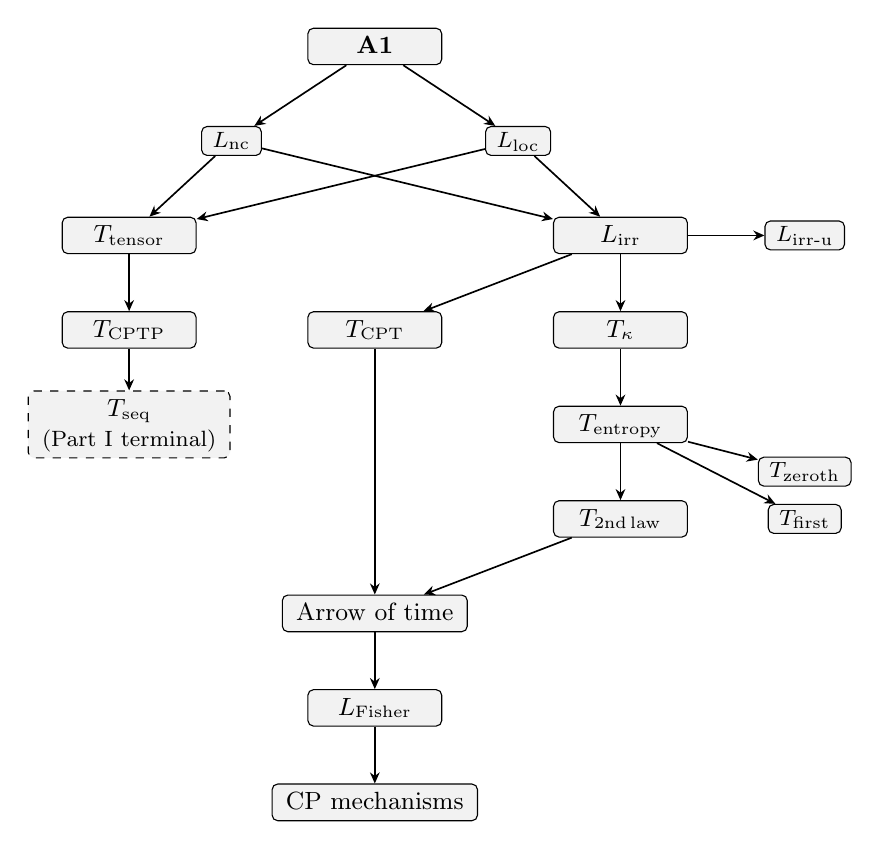
\begin{tikzpicture}[x=2.6cm, y=1.2cm]
  % ---- A1 root ----
  \node[dagbox] at (1.5, 0) (A1) {\textbf{A1}};
  % ---- Shared lemmas ----
  \node[dagsbox] at (0.8,-1) (Lnc)  {$L_{\mathrm{nc}}$};
  \node[dagsbox] at (2.2,-1) (Lloc) {$L_{\mathrm{loc}}$};

  % ---- Part I: dynamics (left, terminal) ----
  \node[dagbox] at (0.3,-2)   (Ttens) {$T_{\mathrm{tensor}}$};
  \node[dagbox] at (0.3,-3)   (TCPTP) {$T_{\mathrm{CPTP}}$};
  \node[dagbox,dashed] at (0.3,-4) (Tseq)  {$T_{\mathrm{seq}}$\\{\footnotesize(Part I terminal)}};

  % ---- Part II / III: entropy + time (right) ----
  \node[dagbox] at (2.7,-2)   (Lirr)  {$L_{\mathrm{irr}}$};
  \node[dagsbox] at (3.6,-2)  (Liu)   {$L_{\mathrm{irr\text{-}u}}$};

  % entropy sub-chain
  \node[dagbox] at (2.7,-3)   (Tkap)  {$T_{\kappa}$};
  \node[dagbox] at (2.7,-4)   (Tent)  {$T_{\mathrm{entropy}}$};
  \node[dagsbox] at (3.6,-4.5)(T0)    {$T_{\mathrm{zeroth}}$};
  \node[dagsbox] at (3.6,-5)  (T1)    {$T_{\mathrm{first}}$};
  \node[dagbox] at (2.7,-5)   (T2nd)  {$T_{\mathrm{2nd\,law}}$};

  % T_CPT: child of L_irr, sibling of entropy chain
  \node[dagbox] at (1.5,-3)   (TCPT)  {$T_{\mathrm{CPT}}$};

  % Convergence
  \node[dagbox] at (1.5,-6)   (Arrow) {Arrow of time};
  \node[dagbox] at (1.5,-7)   (Fish)  {$L_{\mathrm{Fisher}}$};
  \node[dagbox] at (1.5,-8)   (CP)    {CP mechanisms};

  % ---- Edges ----
  \draw[dagarr] (A1)    -- (Lnc);
  \draw[dagarr] (A1)    -- (Lloc);
  % Part I
  \draw[dagarr] (Lnc)   -- (Ttens);
  \draw[dagarr] (Lloc)  -- (Ttens);
  \draw[dagarr] (Ttens) -- (TCPTP);
  \draw[dagarr] (TCPTP) -- (Tseq);
  % Part II entropy chain
  \draw[dagarr] (Lnc)   -- (Lirr);
  \draw[dagarr] (Lloc)  -- (Lirr);
  \draw[dagarr] (Lirr)  -- (Liu);
  \draw[dagarr] (Lirr)  -- (Tkap);
  \draw[dagarr] (Tkap)  -- (Tent);
  \draw[dagarr] (Tent)  -- (T2nd);
  \draw[dagarr] (Tent)  -- (T0);
  \draw[dagarr] (Tent)  -- (T1);
  % T_CPT from L_irr
  \draw[dagarr] (Lirr)  -- (TCPT);
  % Convergence at Arrow
  \draw[dagarr] (T2nd)  -- (Arrow);
  \draw[dagarr] (TCPT)  -- (Arrow);
  \draw[dagarr] (Arrow) -- (Fish);
  \draw[dagarr] (Fish)  -- (CP);
\end{tikzpicture}
\caption{Overview derivation DAG for Paper~3.
\textbf{Part~I} (left, dashed terminal): $L_{\mathrm{nc}}$, $L_{\mathrm{loc}}$
$\to$ $T_{\mathrm{tensor}}$ $\to$ $T_{\mathrm{CPTP}}$ $\to$ $T_{\mathrm{seq}}$.
$T_{\mathrm{seq}}$ is a terminal result of Part~I and does not feed Part~III.
\textbf{Part~II} (right): $L_{\mathrm{irr}}$ generates both the entropy chain
($T_\kappa \to T_{\mathrm{entropy}} \to T_{\mathrm{2nd\,law}}$, with
$T_{\mathrm{zeroth}}$ and $T_{\mathrm{first}}$ as corollaries) \emph{and}
$T_{\mathrm{CPT}}$ (since $L_{\mathrm{irr}} \Rightarrow T$ broken is Step~1 of
$T_{\mathrm{CPT}}$'s proof).
\textbf{Part~III}: $T_{\mathrm{2nd\,law}}$ and $T_{\mathrm{CPT}}$ converge at
the Arrow of time, which yields $L_{\mathrm{Fisher}}$ and the CP mechanisms.
$L_{\mathrm{irr\text{-}u}} \equiv L_{\mathrm{irr\text{-}uniform}}$.}
\label{fig:overview_dag}
\end{figure}


% ======================================================================
\section{Relation to prior work}
\label{sec:related_work}
% ======================================================================

This paper makes a deliberate move that should be stated plainly before the
formal sections begin: it is mostly a \emph{reinterpretation} of well-established
mathematical structures inside a single ``ledger'' vocabulary, not a wholesale
replacement of those structures.  The contribution is a unifying framework
and a small number of derivations that follow from it; the contribution is
not a new mathematics of complete positivity, entropy, horizon thermodynamics,
or information geometry.  This section positions each major claim of Paper~3
against the mainstream literature it draws on, and states explicitly where
the paper is reinterpretive and where it is genuinely additive.

\subsection{CPTP dynamics: Stinespring--Choi--Lindblad--GKSL}

The result that admissibility-preserving evolution is exactly CPTP
($T_{\mathrm{CPTP}}$, \S\ref{sec:cptp}) lives in the orbit of the
Stinespring dilation theorem~\cite{Stinespring1955}, the Choi
characterization of CP linear maps in finite
dimensions~\cite{Choi1975}, and the Lindblad/GKSL generators of completely
positive dynamical semigroups~\cite{Lindblad1976,GKS1976}.  These are
canonical results dating to 1955--1976; the operator-sum/Kraus form is
standard~\cite{Kraus1983}.

Paper~3's contribution here is \emph{provenance}, not endpoint.  The CPTP
class is unchanged.  What changes is the direction of the derivation:
Stinespring proves that every CPTP map admits a dilation; Paper~3 instead
derives the CPTP requirement from A1 + tensor-product structure, with
Stinespring then supplying the Kraus form.  The reader should not expect
$T_{\mathrm{CPTP}}$ to deliver a class of maps outside CPTP, or to supersede
Choi's classification; it should be read as a structural account of why the
CPTP condition holds in this framework.  The Technical Supplement \S 2 makes
the comparison explicit through three differences (derivation direction,
physical interpretation of the dilation, and finite-dimensional restriction).

\subsection{Entropy and the second law: Lieb--Ruskai, Lindblad, Spohn}

The identification of von Neumann entropy with committed capacity
($T_{\mathrm{entropy}}$, \S\ref{sec:entropy}) and the structural derivation
of the second law ($T_{\mathrm{second\,law}}$, \S\ref{sec:secondlaw}) draw
on three lines of established work.  Lieb--Ruskai strong
subadditivity~\cite{LiebRuskai1973} is the entropy-inequality backbone for
monotonicity and data-processing arguments throughout the paper; Wehrl's
review~\cite{Wehrl1978} is the standard reference for general entropy
properties.  Lindblad's CP-map entropy inequalities~\cite{Lindblad1976} and
Spohn's entropy-production framework for quantum dynamical
semigroups~\cite{Spohn1978} are the closest mainstream comparators for the
second-law claim.

Paper~3's reframing here is rhetorical and ontological rather than
mathematical: irreversibility is identified with local unrecoverability of
cross-interface correlations rather than with semigroup thermodynamics.
The outcome --- positive entropy production along admissible trajectories
--- is the same as Spohn's; the route to it is different.  The paper does
\emph{not} present a new entropy inequality of comparable mathematical
independence to Lieb--Ruskai.  What is added is the ledger-accounting
principle (\S\ref{subsec:ledger_accounting}, formalized as a proposition in
Technical Supplement \S 4): the entropy count is robust under small
cost-landscape perturbations because counts do not depend on cost details.

\subsection{Horizon entropy: Bekenstein, Hawking, Gibbons--Hawking, Jacobson}

The geometric carrying-capacity extension (\S\ref{sec:gcc}) and the recovery
of horizon entropy $S_H = A/4$ via the $1/2 \times 1/2$ bookkeeping live in
the lineage of Bekenstein's original information-theoretic black-hole
entropy~\cite{Bekenstein1973}, Hawking's semiclassical particle-creation
result that established horizon thermodynamics as a fact rather than an
analogy~\cite{Hawking1975}, the Gibbons--Hawking extension to cosmological
event horizons in positive-$\Lambda$ spacetimes~\cite{GibbonsHawking1977},
and Jacobson's derivation of the Einstein equation as an equation of state
from horizon thermodynamics~\cite{Jacobson1995}.  The holographic principle
of 't Hooft and Susskind~\cite{tHooft1993,Susskind1995} sits in the
background as the area-law commitment.

Paper~3's contribution here is \emph{combinatorial accounting}, not new
gravitational physics.  The $S = A/4$ area law is unchanged; the
$1/2 \times 1/2$ decomposition (relational symmetrization $\times$
Hamiltonian-constraint redundancy, formalized in Technical Supplement \S 6
under hypothesis H2) is a specific bookkeeping account of where the standard
$1/4$ prefactor comes from.  The claim that thermodynamic entropy,
entanglement entropy, and horizon entropy are three specializations of one
ACC-saturation count is a unifying re-reading; it does not predict horizon
phenomena outside the Bekenstein--Hawking--Gibbons--Hawking framework.  The
de Sitter combinatorial value $S_{dS} = 61\ln 102 \approx 282.12$ nats is
specifically a Gibbons--Hawking-style cosmological-horizon entropy, with the
$C_{\mathrm{total}} = 61$ count inherited from Paper~2 rather than derived
in Paper~3.

\subsection{Fisher information and the renormalization group: Braunstein--Caves, Petz, Bény--Osborne}

The Fisher-information section (\S\ref{sec:fisher}) draws on the quantum
Fisher metric of Braunstein and Caves~\cite{BraunsteinCaves1994}, the
classification of monotone metrics by Petz~\cite{Petz1996}, and the
foundational information-geometry framework of Amari and
Nagaoka~\cite{AmariNagaoka2000}.  The closest external support for the
``RG flow as Fisher gradient descent'' claim is the program of B\'eny and
Osborne~\cite{BenyOsborne2015}, who formulate RG explicitly as a family of
quantum channels with an induced information geometry on the space of
admissible effective descriptions.

Paper~3's contribution here is the capacity-count normalization
($S = (d_{\mathrm{eff}}/2)\ln\det G$ with $d_{\mathrm{eff}} = 102$ from
Paper~2) and the suggestion that this same Fisher gradient feeds the
channel-crossing structure of Paper~4's flavor sector.  The
information-geometric RG program itself is not new to this paper; the
specific embedding of APF capacity counting into that program is.

\subsection{Reconstruction programs: Hardy, CDP, Masanes--M\"uller, Daki\'c--Brukner}

This paper sits stylistically in the family of operational quantum
reconstruction programs --- Hardy's five reasonable axioms~\cite{Hardy2001},
the informational derivation of Chiribella, D'Ariano, and
Perinotti~\cite{CDP2011}, the derivation of Masanes and
M\"uller~\cite{MM2011}, and the entanglement-special argument of Daki\'c
and Brukner~\cite{DakicBrukner2009}.  Compared to these programs, the
APF inventory (PLEC's four components A1, MD, A2, BW plus FD1--FD6
constitutive principles, taken from Paper~1) is comparable to or lighter
than peer inventories.  The departure from the reconstruction tradition is
scope: the APF program attempts not just quantum kinematics but also
thermodynamics, horizons, flavor, and cosmology.  That broader ambition is
both this paper's distinctive feature and its largest source of
proof-burden.

\subsection{Arrow of time: Maccone, Caticha, Chen, Di Biagio, Buchholz}

The structural account of the arrow of time
(\S\S\ref{sec:secondlaw}--\ref{sec:arrow}, especially the rebuttal of the
typicality framing in
\S\ref{subsec:arrow_restricted_phasespace}) lands in a contested foundational
literature.  Several non-equivalent recent treatments offer alternative
escapes from the typicality framing:
Maccone's information-theoretic unrecordability~\cite{Maccone2009};
Caticha's entropic-dynamics inference~\cite{Caticha2011};
Chen's initial-state-realism approach~\cite{Chen2019};
the operational-asymmetry framework of Di Biagio, Don\`a, and
Rovelli~\cite{DiBiagio2021};
the algebraic-QFT framework of Buchholz and Yngvason~\cite{Buchholz2023}.
Paper~3's resolution is constraint-on-the-admissible-set: low initial entropy
is reframed as a small initial admissible set whose size is computable from
A1, not as one improbable draw from a uniform measure.  This is closer in
spirit to Caticha and Chen than to Maccone's unrecordability or Buchholz's
algebraic-QFT framing.

\subsection{CP violation: Jarlskog and the empirical anchor at T2K}

The CP-violation section (\S\ref{sec:cp}) proposes two structurally distinct
mechanisms: holonomy phases (CKM-like) and entropy-optimization phases
(PMNS-like).  The mainstream structural treatment of CP violation is the
invariant-CP program of Jarlskog~\cite{Jarlskog2005,Jarlskog2012}, which
phrases CP-violation in basis-independent terms via invariants of the mass
matrices.  The two-mechanism split offered here is not Jarlskog's result;
it belongs to the same broader effort to phrase CP-violation
basis-independently.  Where Jarlskog gives invariant algebraic structures,
Paper~3 offers geometric-holonomy and entropy-extremization mechanisms.

The numerical phases ($\delta_{\mathrm{CKM}} \approx 1.16$ rad,
$\delta_{\mathrm{PMNS}}$ specific value) are deferred to Paper~4.  The
empirical anchor that any sequel claim about $\delta_{\mathrm{PMNS}}$ will
ultimately have to meet is the long-baseline neutrino-oscillation programme,
of which the T2K Collaboration's 2020 \emph{Nature} measurement of
$\delta_{CP}$~\cite{T2K2020} is currently the strongest published constraint.
The structural treatment in this paper is therefore not free-floating; it has
a real target surface.

\subsection{What this section does not do}

This section positions Paper~3 in the established literature.  It does not
claim that Paper~3 supersedes any of the works cited.  Specifically:

\begin{itemize}
    \item $T_{\mathrm{CPTP}}$ is a reinterpretation of standard CP-map theory, not a replacement.
    \item $T_{\mathrm{entropy}}$ uses the standard Lieb--Ruskai monotonicity backbone; the contribution is the cost-interpretation, not a new entropy inequality.
    \item $S_H = A/4$ is the standard Bekenstein--Hawking--Gibbons--Hawking area law; the contribution is the $1/2 \times 1/2$ bookkeeping decomposition.
    \item RG-as-Fisher-descent is directionally aligned with B\'eny--Osborne; the contribution is the capacity-count normalization.
    \item The two-mechanism CP framing belongs in conversation with Jarlskog's invariant-CP program; the contribution is the structural separation, not the invariant structure.
\end{itemize}

\noindent The reader should encounter the formal sections that follow with this
context in mind.  The framework is unifying; the constituent results are
mostly familiar; the genuine novelty lies in their joint reorganization
under finite-enforcement bookkeeping.


% ======================================================================
\section{Part I: Admissible Dynamics}
% ======================================================================

\setcounter{subsection}{0}

\begin{tcolorbox}[apfbox, title={Operational primitives: where each ledger term is defined and used}]
Paper~3 takes Paper~1's static admissibility structure (A1 + PLEC + tensor products $T_{\mathrm{tensor}}$) and Paper~2's capacity counting ($C_{\mathrm{total}} = 61$, $d_{\mathrm{eff}} = 102$) as inputs.  Five operational primitives carry the dynamical and entropic argument that follows.  This box is a wayfinder, not new content; every claim points to where the term is defined or formalized.

\begin{description}[topsep=2pt,itemsep=2pt]
  \item[Ledger.]  The bookkeeping of committed enforcement cost across an interface.  ``Committed'' means capacity that cannot be locally reclaimed once spent.  \emph{Used as organizing metaphor throughout;} \emph{formalized in two specific ways:} (i) entropy as committed-capacity count ($T_{\mathrm{entropy}}$, \S\ref{sec:entropy}); (ii) ACC as the geometric specialization (\S\ref{sec:gcc}).  \emph{Foundational discussion:} \S\ref{sec:related_work}.
  \item[CPTP map.]  An admissibility-preserving evolution.  \emph{Derived as theorem (not definition):} $T_{\mathrm{CPTP}}$ (\S\ref{sec:cptp}); standard mathematical content from Stinespring--Choi--Lindblad--GKSL is reinterpreted, not replaced (see \S\ref{sec:related_work}).
  \item[Committed capacity / cross-interface correlation.]  Capacity that has been allocated to a correlation across two interfaces.  Once committed, it cannot be reclaimed by any local operation at one interface.  \emph{Formalized:} $L_{\mathrm{irr}}$ (\S\ref{sec:arrow}).  \emph{Quantitative form:} $\kappa = 2$ multiplier of $T_\kappa$ (\S\ref{sec:entropy}); entropy as the count of such commitments via $T_{\mathrm{entropy}}$ (\S\ref{sec:entropy}).
  \item[Admissibility carrying capacity (ACC).]  The general-interface capacity concept of which enforcement cost is the quantum-interface specialization.  An ACC interface may be a quantum bipartition, a causal horizon, or a cosmological boundary.  \emph{Defined and developed:} \S\ref{sec:gcc}.  \emph{Specializations:} (i) horizon entropy $S = A/4$ via the $1/2 \times 1/2$ bookkeeping; (ii) de~Sitter $S_{dS} = 61\ln 102$ via $C_{\mathrm{total}}$ and $d_{\mathrm{eff}}$ from Paper~2.
  \item[Constraint functional $\Phi_c$.]  The dimensionless excess between unconstrained and admissible mode counts: $\Phi_c = \ln(d_{\mathrm{field}}/d_{\mathrm{admissible}})$.  Monotone-non-increasing along admissible cosmological trajectories under hypothesis H3 (Technical Supplement).  \emph{Defined:} \S\ref{sec:cosmogenesis}.  \emph{Used:} the staged-relaxation cosmogenesis picture (\S\ref{sec:cosmogenesis}); the macroscopic-arrow argument (\S\ref{sec:arrow}, closing).
\end{description}

\noindent The Technical Supplement provides full formal treatments and the operational protocol for measuring committed capacity from physical observables.
\end{tcolorbox}

% ======================================================================
\section{Complete Positivity as a Theorem ($T_{\mathrm{CPTP}}$)}
\label{sec:cptp}
% ======================================================================

Paper~1 established that admissibility-preserving maps must be
trace-preserving and positive: the trace is committed capacity normalized to
one, and maps that fail positivity produce states with negative enforcement
costs, which are inadmissible.  What Paper~1 left conditional was the step
from positivity to \emph{complete} positivity.

The distinction matters.  A map $\Phi$ on a system $S$ is positive if it
maps valid density matrices to valid density matrices.  It is completely
positive if $\Phi\otimes\mathbb{1}_R$ is also positive for any ancilla system
$R$ evolved by the identity map.  The difference is ancilla-stability: a
merely positive (but not completely positive) map can produce unphysical
states when the system is entangled with a reference system that does not
evolve.

Paper~1 deferred this step because ancilla-stability requires the tensor
product structure ($T_{\mathrm{tensor}}$) to be in place, and requires an
analysis of how admissible maps compose when the ancilla carries its own
enforcement budget.  Both prerequisites are now available.

\begin{tcolorbox}[apfbox, title={Theorem $T_{\mathrm{CPTP}}$ (Complete Positivity) \epitag{P}}]
\textbf{Statement.}
Let $\Phi: \mathcal{B}(\mathcal{H}_S) \to \mathcal{B}(\mathcal{H}_S)$ be any
map that preserves admissibility of the enforcement regime at interface
$\Gamma_S$.  Then $\Phi$ is completely positive and trace-preserving (CPTP),
and admits a Kraus decomposition
\[
  \Phi(\rho) = \sum_k K_k\,\rho\,K_k^\dagger, \qquad
  \sum_k K_k^\dagger K_k = \mathbb{1}.
\]

\textbf{Variables:}
\begin{varlist}
  \item $\mathcal{H}_S$ --- Hilbert space of the system at interface $\Gamma_S$
  \item $K_k$ --- Kraus operators; $k$ indexes the environment outcomes
  \item $\rho$ --- density matrix of the system
\end{varlist}

\textbf{Proof (three steps).}

\smallskip\noindent\textit{Step~1 (Trace preservation).}
A1 fixes $C(\Gamma_S)$ as a finite, positive constant: the enforcement budget
at interface $\Gamma_S$.  The trace $\mathrm{tr}\,\rho = 1$ is the
normalization of that budget ($C_{\mathrm{active}}/C(\Gamma_S) = 1$).  An
admissibility-preserving map redistributes committed capacity among states but
cannot alter $C(\Gamma_S)$ itself --- doing so would change the enforcement
budget, which is precisely the datum A1 fixes.  Hence:
\begin{itemize}[nosep]
  \item If $\mathrm{tr}\,\Phi(\rho) > 1$: capacity has been created.  A1
    violation (budget exceeds its fixed value).
  \item If $\mathrm{tr}\,\Phi(\rho) < 1$: capacity has been annihilated.
    A1 violation equally (budget falls below its fixed value; A1 requires
    positivity \emph{and} conservation of the budget, not merely an upper
    bound).
\end{itemize}
Therefore $\mathrm{tr}\,\Phi(\rho) = 1$ unconditionally, with A1 as the sole
source.  ($L_{\mathrm{irr}}$ is not needed here; it enters only in Step~2.)

\smallskip\noindent\textit{Step~2 (Complete positivity via ancilla-stability).}
By $T_{\mathrm{tensor}}$ (Paper~1), the joint system $S\otimes R$ for any
ancilla $R$ carries an independent enforcement budget $C(\Gamma_R)$.  The
state $\rho_{SR}$ is admissible if and only if it has non-negative
enforcement costs at all interfaces.  Now apply $\Phi\otimes\mathbb{1}_R$:
$\Phi$ acts on $\Gamma_S$ and the identity acts on $\Gamma_R$.  Since
$\Gamma_R$ is independent of $\Gamma_S$ (by $L_{\mathrm{loc}}$), the
evolution at $\Gamma_S$ cannot create inadmissible states at $\Gamma_R$.
The joint map therefore preserves admissibility of $\rho_{SR}$ for any
initial $\rho_{SR} \geq 0$.  This is the definition of complete positivity.

\smallskip\noindent\textit{Step~3 (Kraus representation).}
Given that $\Phi$ is CPTP, the Stinespring dilation theorem~\cite{Stinespring1955}
applies: there exists a Hilbert space $\mathcal{H}_E$ (the environment) and an isometry
$V: \mathcal{H}_S \to \mathcal{H}_S\otimes\mathcal{H}_E$ such that
$\Phi(\rho) = \mathrm{tr}_E[V\rho V^\dagger]$.  The Kraus operators~\cite{Choi1975,Kraus1983} are
$K_k = (\mathbb{1}_S\otimes\langle k|_E)V$ for any orthonormal basis
$\{|k\rangle\}$ of $\mathcal{H}_E$.

\textbf{Enforcement interpretation of the dilation.}  The Stinespring
isometry $V$ describes the system and environment evolving unitarily, with
each maintaining a separate enforcement budget.  The partial trace over $E$
discards the environmental budget: $L_{\mathrm{irr}}$ ensures that the
capacity committed to $S$--$E$ correlations cannot be recovered at $\Gamma_S$,
so tracing out $E$ is not an approximation but the exact enforcement account.

\coderef{check\_T\_CPTP}{core.py}
\end{tcolorbox}

\smallskip\noindent\textbf{Remark on Paper~1's conditional statement.}
Paper~1 listed $T_{\mathrm{CPTP}}$ as conditional on the identification
``ancilla-stability: coupling to an ancilla preserves admissibility.''  That
identification is now a theorem: Step~2 above derives it from
$T_{\mathrm{tensor}}$ and $L_{\mathrm{loc}}$.  The conditional flag on
$T_{\mathrm{CPTP}}$ in Paper~1's Table~H.1 is accordingly lifted.

\smallskip\noindent\textbf{What $T_{\mathrm{CPTP}}$ does not say.}
The theorem characterizes the \emph{class} of admissible evolution maps.  It
does not specify which map is selected in any given physical situation; that
requires the dynamical structure developed in Paper~6 (Euler-Lagrange and
geodesic equations from enforcement cost extremization).

\subsection{Sequential composition and the no-bit-commitment corollary}
\label{sec:seq}

\begin{tcolorbox}[apfbox, title={Theorem $T_{\mathrm{seq}}$ (Sequential Admissibility) \epitag{P}}]
\textbf{Statement.}
Composites of admissible CPTP maps are admissible CPTP maps.  For $T$ time
steps, the cumulative enforcement cost is bounded:
\[
  \sum_{t=1}^{T} \varepsilon(d_t) \;\leq\; C(\Gamma)\cdot T.
\]
Time-evolved observables $a(t) = U_t^\dagger\,a\,U_t$ satisfy the same
Cirel'son operator identity as static observables, giving the Tsirelson bound
$2\sqrt{2}$ for temporal CHSH correlators.

\textbf{Proof.}  CPTP maps form a semigroup under composition: the composite
of two trace-preserving maps is trace-preserving, and the composite of two
completely positive maps is completely positive (tensor product of Kraus
operators).  This is the standard GKSL--Lindblad picture~\cite{Lindblad1976,GKS1976}
interpreted via the enforcement ledger.  The cost bound follows because each
step draws at most $\varepsilon(d_t) \leq C(\Gamma)$ from the budget; the
total over $T$ steps is bounded by $C(\Gamma)\cdot T$ by subadditivity.

For the dynamic Tsirelson bound: the Cirel'son identity
$\|[a(t_1), a(t_2)]\| \leq 2$ holds for any two unitary-evolved $\pm 1$
observables because unitary conjugation is an automorphism of the operator
algebra, and the norm bound $\|[a,b]\| \leq 2\|a\|\|b\|$ is algebraic, not
state-dependent.  The Tsirelson bound for temporal correlators follows from
the same Cirel'son identity as for static ones.
\end{tcolorbox}

\medskip\noindent\textbf{Corollary block: no-cloning, no-deleting, no-bit-commitment.}

Three constraints on information processing follow immediately from
$T_{\mathrm{CPTP}}$ and the capacity accounting of $C(\Gamma) = 61$.

\smallskip\noindent\emph{No-cloning.}  A perfect cloning map would send
$\rho\mapsto\rho\otimes\rho$.  This doubles the enforcement demand at
$\Gamma_S$: the output requires $2\,C(\Gamma)$ to maintain.  Since A1 fixes
$C(\Gamma)$, the map is inadmissible.  More formally, a cloning map cannot
be CPTP because it is not linear: for $\rho = p\rho_1+(1-p)\rho_2$, the
cloning map gives $\rho^{\otimes 2}$, which differs from
$p\rho_1^{\otimes 2}+(1-p)\rho_2^{\otimes 2}$ unless the states are orthogonal.
CPTP maps are linear; cloning is not.

\smallskip\noindent\emph{No-deleting.}  Deletion of one copy from
$\rho\otimes\rho$ would require a map that reduces the environmental record
at $\Gamma_E$.  But $L_{\mathrm{irr}}$ prohibits local erasure of
cross-interface correlations.  The deletion map is inadmissible.

\smallskip\noindent\emph{No-bit-commitment.}  A bit-commitment protocol
requires: (i) \emph{hiding} --- the receiver cannot determine the committed
bit $b$ from the committed state $\rho_b$; and (ii) \emph{binding} --- the
committer cannot change $b$ after commitment.  These two requirements are
jointly inadmissible.  If hiding holds then $\rho_0^R = \rho_1^R$ (the
receiver's reduced state is identical for both bits).  By Uhlmann's theorem
plus the Stinespring dilation supplied by $T_{\mathrm{CPTP}}$, the joint
purified states satisfy $|\psi_1\rangle = (U_C\otimes\mathbb{1}_R)|\psi_0\rangle$
for some unitary $U_C$ on the committer's system.  But $U_C$ is a CPTP map
(unitary evolution is a special case), so the committer can apply it after
commitment, transforming $\rho_0$ into $\rho_1$: binding fails.  Hence hiding
$\Rightarrow$ not binding, and no protocol achieves both simultaneously.


% ======================================================================
\section{Part II: The Ledger}
% ======================================================================

\setcounter{subsection}{0}

% ======================================================================
\section{Entropy as Committed Capacity ($T_{\mathrm{entropy}}$, $T_{\kappa}$)}
\label{sec:entropy}
% ======================================================================

Paper~1 introduced the von Neumann entropy functional~\cite{vonNeumann1932}
as a consequence of the operator algebra, but left its physical interpretation
informal: entropy was described as measuring ``how much has been committed.''
This section makes that identification precise, derives the directed-enforcement
multiplier $\kappa = 2$ that controls the cost of each commitment, and shows that
the standard laws of thermodynamics follow immediately.  The strong-subadditivity
infrastructure that supports monotonicity and data-processing arguments throughout
what follows is the Lieb--Ruskai backbone~\cite{LiebRuskai1973,Wehrl1978}.

The approach is bottom-up.  We first establish that the cost per
distinction cannot be $\kappa = 1$ (single-interface commitment is erasable)
and cannot be $\kappa > 2$ (a third independent interface commitment would
require a second environment, which is a new correlation, not an additional
cost on the original one).  The unique value is $\kappa = 2$.

The derivation chain for this section is shown below.

\begin{center}
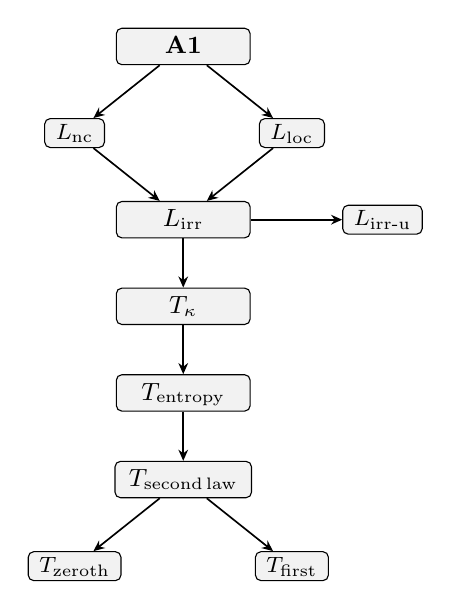
\begin{tikzpicture}[x=2.3cm, y=1.1cm]
  % Row 0
  \node[dagbox] at (1,0) (A1) {\textbf{A1}};
  % Row 1
  \node[dagsbox] at (0.4,-1) (Lnc)  {$L_{\mathrm{nc}}$};
  \node[dagsbox] at (1.6,-1) (Lloc) {$L_{\mathrm{loc}}$};
  % Row 2
  \node[dagbox] at (1,-2) (Lirr)   {$L_{\mathrm{irr}}$};
  \node[dagsbox] at (2.1,-2) (Liu) {$L_{\mathrm{irr\text{-}u}}$};
  % Row 3
  \node[dagbox] at (1,-3) (Tkap)   {$T_{\kappa}$};
  % Row 4
  \node[dagbox] at (1,-4) (Tent)   {$T_{\mathrm{entropy}}$};
  % Row 5
  \node[dagbox] at (1,-5) (T2nd)   {$T_{\mathrm{second\,law}}$};
  % Row 6
  \node[dagsbox] at (0.4,-6) (T0)  {$T_{\mathrm{zeroth}}$};
  \node[dagsbox] at (1.6,-6) (T1)  {$T_{\mathrm{first}}$};
  % Edges
  \draw[dagarr] (A1)   -- (Lnc);
  \draw[dagarr] (A1)   -- (Lloc);
  \draw[dagarr] (Lnc)  -- (Lirr);
  \draw[dagarr] (Lloc) -- (Lirr);
  \draw[dagarr] (Lirr) -- (Liu);
  \draw[dagarr] (Lirr) -- (Tkap);
  \draw[dagarr] (Tkap) -- (Tent);
  \draw[dagarr] (Tent) -- (T2nd);
  \draw[dagarr] (T2nd) -- (T0);
  \draw[dagarr] (T2nd) -- (T1);
\end{tikzpicture}
\end{center}

\smallskip

\begin{tcolorbox}[apfbox, title={Theorem $T_{\kappa}$ (Directed Enforcement Multiplier) \epitag{P}}]
\textbf{Statement.}
The directed enforcement multiplier is $\kappa = 2$.  Each maintained
distinction incurs exactly two independent interface commitments: one at the
system interface $\Gamma_S$ (forward stabilization) and one at the
environment interface $\Gamma_E$ (environmental record).

\textbf{Proof.}

\smallskip\noindent\emph{Lower bound $\kappa \geq 2$.}
Step~1: $L_{\mathrm{nc}}$ requires forward enforcement at $\Gamma_S$ ---
without active stabilization, distinctions collapse.  This commits at least
$\varepsilon$ at $\Gamma_S$ per distinction.  Step~2: $L_{\mathrm{irr}}$
requires that when a system creates a distinction, the $S$--$E$ correlation
($\Delta > 0$) commits capacity at $\Gamma_E$ independently.  This is the
environmental record.  Step~3: by $L_{\mathrm{loc}}$, $\Gamma_S$ and
$\Gamma_E$ are independent budgets.  Freeing $C_{\mathrm{fwd}}$ at $\Gamma_S$
does not free $C_{\mathrm{env}}$ at $\Gamma_E$.  The two commitments are
structurally distinct.  Total cost $\geq 2\varepsilon$ per distinction, so
$\kappa \geq 2$.

\smallskip\noindent\emph{Upper bound $\kappa \leq 2$.}
A third commitment would require a third independent interface --- a second
environment.  But a second environment constitutes a new distinction (the
cross-interface correlation between the two environments), not an additional
enforcement obligation on the original distinction.  PLEC's argmin
component (A2, the minimum-cost selection feature of the admissibility
variational principle --- enforce exactly what is needed to maintain
admissibility, no more) then gives $\kappa \leq 2$.

\smallskip\noindent\emph{Uniqueness.}  $\kappa \geq 2$ and $\kappa \leq 2$
together give $\kappa = 2$.

\textbf{Physical interpretation.}  $\kappa = 2$ is the enforcement analogue
of the Nyquist sampling theorem: two independent samples (system and
environment) are required to fully characterize a distinction's enforcement
state.  The environment is the independent auditor.

\coderef{check\_T\_kappa}{core.py}
\end{tcolorbox}

With $\kappa = 2$ in hand, the identification of entropy with committed
capacity becomes sharp.

\begin{tcolorbox}[apfbox, title={Theorem $T_{\mathrm{entropy}}$ (Von~Neumann Entropy as Committed Capacity) \epitag{P}}]
\textbf{Statement.}
The entropy $S(\Gamma, t) = \mathcal{E}_\Gamma(R_{\mathrm{active}}(t))$,
defined as the enforcement demand of active correlations at interface
$\Gamma$, equals the von~Neumann entropy $S(\rho) = -\mathrm{tr}(\rho\log\rho)$
in any quantum-admissible regime.

The entropy satisfies five properties, all derived from capacity structure:
\begin{enumerate}[nosep]
\item $S \geq 0$ (enforcement costs are non-negative).
\item $S = 0$ if and only if $\rho$ is pure (no committed capacity beyond
  the minimum).
\item $S \leq \log d$ with equality at maximal mixing (capacity saturation).
\item Subadditivity: $S(AB) \leq S(A) + S(B)$ (non-closure bounds joint
  enforcement).
\item Concavity: $S(\sum_i p_i\rho_i) \geq \sum_i p_i S(\rho_i)$ (mixing
  never decreases committed capacity).
\end{enumerate}

\textbf{Proof.}  The identification $S = -\mathrm{tr}(\rho\log\rho)$ follows
from the uniqueness of the capacity cost function $F(d) = d$ (proved via
Cauchy's functional equation in Paper~2, $L_{\mathrm{Cauchy}}$) together
with the spectral decomposition $\rho = \sum_i \lambda_i |i\rangle\langle i|$:
the cost of maintaining $n$ orthogonal distinctions weighted by $\lambda_i$
is $-\sum_i \lambda_i \log\lambda_i = -\mathrm{tr}(\rho\log\rho)$.
Properties~1--3 are direct from capacity non-negativity and the
$[0, \log d]$ range of committed fractions.  Property~4 (subadditivity)
follows from $L_{\mathrm{nc}}$: non-closure means joint enforcement at a
shared interface exceeds individual costs, but the excess $\Delta > 0$
forces $S(AB) \leq S(A) + S(B)$ via the data-processing inequality.
Property~5 (concavity) follows because mixing increases the number of
distinctions being simultaneously maintained.

\coderef{check\_T\_entropy}{core.py}
\end{tcolorbox}

\subsection{The ledger-accounting principle}
\label{subsec:ledger_accounting}

The entropy just derived is a \emph{count} of the microscopic configurations
consistent with the ledger's cost constraints---nothing more.  This is a
deep structural feature, not a convenience.  The multiplicity of admissible
configurations depends on the cardinality of the admissible set, not on the
detailed cost landscape that defines it.  Two consequences follow.

First, interaction corrections that shift the energy of the saturated
configuration leave the configuration count invariant: interactions modify
which state is lowest-cost, but the count of admissible states above that
minimum is unchanged.  Second, thermal corrections that alter the relative
weights of states with different costs also leave the saturated count
invariant, because at saturation every admissible configuration has been
realized and there are no unrealized states to reweight.

This is the key to the exactness of the cosmological entropy bound: the
de~Sitter entropy $S_{dS} = C_{\mathrm{total}}\,\ln d_{\mathrm{eff}}
= 61\ln 102$ is not a leading-order approximation refined by interactions;
it is a combinatorial identity in the admissible set.  The cosmological
horizon to which this identity attaches is the Gibbons--Hawking
horizon~\cite{GibbonsHawking1977} of a positive-$\Lambda$ de~Sitter
spacetime; the combinatorial value $61\ln 102$ is interpreted as the
ACC-saturation entropy of that horizon, with the count $C_{\mathrm{total}} = 61$
inherited from Paper~2's capacity-partitioning argument.  This is therefore
a structural cosmological-entropy claim within the
Bekenstein--Hawking--Gibbons--Hawking framework, not a competitor to it.  The thermodynamic
formalism (partition function, finite-temperature corrections to the
free energy, beta-dependence of individual observables) is developed in
Paper~7; Paper~3 needs only the accounting principle itself.  We return to
the point in~\S\ref{subsec:gcc_unify}, where the same accounting unifies
thermodynamic, entanglement, and horizon entropy as three views of
interface-capacity saturation.

\subsection{Thermodynamic laws as corollaries}

The zeroth and first laws of thermodynamics follow from $T_{\mathrm{entropy}}$
and $L_{\mathrm{irr}}$ without additional assumptions.

\begin{tcolorbox}[apfbox, title={Theorem $T_{\mathrm{zeroth}}$ (Zeroth Law) \epitag{P}}]
\textbf{Statement.}  Define the inverse temperature $\beta = \log d / \varepsilon$
and the temperature $T = \varepsilon / \log d$.  Capacity flows spontaneously
from high-$T$ (low-$\beta$) to low-$T$ (high-$\beta$) interfaces.
Equilibrium is the state $\beta_1 = \beta_2$, and this condition is
transitive: if $\Gamma_1$ is in equilibrium with $\Gamma_2$, and $\Gamma_2$
with $\Gamma_3$, then $\Gamma_1$ is in equilibrium with $\Gamma_3$.

\textbf{Derivation.}  Transfer of one unit from $\Gamma_2$ to $\Gamma_1$
changes entropy by $\Delta S = (\beta_1 - \beta_2)\varepsilon$.  By
$L_{\mathrm{irr}}$, entropy-increasing transfers are spontaneous; flow stops
when $\beta_1 = \beta_2$.  Transitivity is transitivity of real-number equality.
The cosmological equilibrium temperature is $T_{\mathrm{univ}} = \varepsilon/\log 102$.

\coderef{check\_T\_zeroth\_law}{supplements.py}
\end{tcolorbox}

\begin{tcolorbox}[apfbox, title={Theorem $T_{\mathrm{first}}$ (First Law) \epitag{P}}]
\textbf{Statement.}  Energy changes at any interface decompose as
$dE = dQ + dW$, where $dQ = T\,dS$ (heat: irreversible, entropy-producing,
forced by $L_{\mathrm{irr}}$) and $dW = dE - T\,dS$ (work: reversible,
entropy-neutral).

\textbf{Derivation.}  $L_{\mathrm{irr}}$ partitions any $dE$ into
irreversible (commitment-generating) and reversible (commitment-neutral)
components.  Pure commitment: $dQ = T\,dS,\; dW = 0$.  Pure work: $dQ = 0,\;
dW = dE$.  The mixed case is the accounting identity $dE = dQ + dW$.
For the cosmological fill through all 61 capacity types, every commitment is
pure heat ($dW_{\mathrm{total}} = 0$): the universe does no work on itself
during the capacity fill.

\coderef{check\_T\_first\_law}{supplements.py}
\end{tcolorbox}


% ======================================================================
\section{The Second Law ($T_{\mathrm{second\,law}}$)}
\label{sec:secondlaw}
% ======================================================================

The second law is the claim that entropy does not decrease.  In statistical
mechanics this is usually derived from typicality arguments or taken as a
boundary condition on the initial state.  The closest operator-algebraic
treatment is Spohn's positive-entropy-production framework for quantum
dynamical semigroups~\cite{Spohn1978}, which establishes approach to
equilibrium from completely positive evolution and is the mainstream
comparator for the result below.  In the admissibility framework the
second law is derived not from semigroup thermodynamics but from
$L_{\mathrm{irr}}$: the local unrecoverability of cross-interface
correlations.  The outcome --- positive entropy production along admissible
trajectories --- agrees with Spohn; the route is different, and the
substantive novelty is the rhetorical shift rather than a replacement of
the monotonicity result itself (see \S\ref{sec:related_work}).

\begin{tcolorbox}[apfbox, title={Theorem $T_{\mathrm{second\,law}}$ (Second Law of Thermodynamics) \epitag{P}}]
\textbf{Statement.}  The entropy of any closed subsystem is non-decreasing
under admissibility-preserving evolution.  The entropy of the universe is
strictly increasing during the capacity fill and constant at saturation.

\medskip\noindent\textbf{Level~A: Subsystem second law.}

For any CPTP map $\Phi$ arising from tracing over an environment that begins
in a low-entropy state:
\[
  S(\Phi(\rho_S)) \;\geq\; S(\rho_S).
\]

\textit{Proof.}  By $T_{\mathrm{tensor}}$, the total system-environment
evolution is unitary: $S(\rho_{SE}(t)) = S(\rho_{SE}(0))$ (unitary evolution
is entropy-preserving).  By $L_{\mathrm{irr}}$, the partial trace over $E$
discards cross-interface correlations that cannot be recovered at $\Gamma_S$.
Information about $S$ that has leaked to $E$ is gone from the perspective of
any $S$-local observer.  The data-processing inequality then gives
$S(\Phi(\rho_S)) = S(\mathrm{tr}_E[\rho_{SE}(t)]) \geq S(\rho_S)$ for
unital channels; strict inequality holds whenever new correlations form.

\medskip\noindent\textbf{Level~B: Cosmological second law.}

Define the $k$-step entropy $S(k) = k\ln d_{\mathrm{eff}} = k\ln 102$ for
$k \in \{0, 1, \ldots, 61\}$ capacity types committed.  Then:
\begin{enumerate}[nosep]
\item $S(k)$ is strictly increasing: $S(k+1) - S(k) = \ln 102 > 0$.
\item $L_{\mathrm{irr}}$ makes $k$ non-decreasing in time: committed types
  cannot be uncommitted by any local operation.
\item Therefore $dS/dt \geq 0$ globally, with equality only at saturation
  $k = 61$.
\item At saturation: $S = S_{dS} = 61\ln 102 \approx 282.12$ nats $= S_{\max}$.
\end{enumerate}

\medskip\noindent\textbf{Not a boundary condition.}  The standard derivation
of the second law in statistical mechanics requires either a special
low-entropy initial state (the ``past hypothesis'') or a Boltzmann-style
typicality argument.  Neither is needed here.  $L_{\mathrm{irr}}$ gives
irreversibility as a structural consequence of A1, $L_{\mathrm{nc}}$, and
$L_{\mathrm{loc}}$ without any assumption about initial conditions.  The
capacity fill begins at $k=0$ (the empty ledger) and proceeds to $k=61$
because each commitment is irreversible.  The initial low-entropy state is
not assumed; it is forced by the fact that no capacity had yet been committed.

\coderef{check\_T\_second\_law}{supplements.py}
\end{tcolorbox}


% ======================================================================
\section{Geometric Carrying Capacity}
\label{sec:gcc}
% ======================================================================

The ledger developed in \S\S\,\ref{sec:entropy}--\ref{sec:secondlaw} tracks
the cost of maintaining distinction across a \emph{quantum} interface: a
bipartition of a pure state into system and environment, or the interface
between a system and its purifying ancilla.  We now extend the framework to
general relational interfaces, including causal and cosmological ones.  The
extension is natural: every interface carries an admissibility capacity---an
upper bound on the number of independent relational degrees of freedom that
can be coordinated across it---and saturation of this capacity is the
universal condition under which entropy attains its characteristic scaling.

\subsection{From enforcement cost to interface capacity}
\label{subsec:gcc_cost_to_capacity}

For a quantum interface, the capacity is the dimension of the relevant
tensor factor and the cost is the enforcement cost $\varepsilon^*$ per
distinction maintained.  For a causal interface---a horizon---or a
cosmological boundary, the capacity is bounded by the geometric area of the
interface in Planck units, and the cost is the enforcement cost of
maintaining a distinction accessible at that interface.  We call the general
upper bound the \emph{admissibility carrying capacity} (ACC) of the
interface.  The ACC is an upper bound, not a state; it plays the same role
that enforcement capacity plays in Paper~1 and the same role that
$C_{\mathrm{total}}$ plays in the cosmological bookkeeping of Paper~2.
What counts as ``enforcement'' is the maintenance of relational distinction
across the interface; what counts as ``saturation'' is the condition that
the number of admissible distinctions equals the ACC.

This extension is not a new axiom.  It follows from A1 (finite capacity
applies to every enforcement problem) and the observation that an interface
with finite geometric extent can only support finitely many independent
relational distinctions.  The full derivation---showing that the geometric
bound is Bekenstein area-law in structure---is developed in Paper~5 and
Paper~6 (spacetime and gravity); here we take it as given and focus on the
entropic consequences.

\subsection{Relational bookkeeping: the two factors of one-half}
\label{subsec:gcc_bookkeeping}

Two factors of $1/2$ must be applied to the naive ACC count when converting
an interface area into an entropy.  They have a principled origin and are
not free parameters.

\smallskip\noindent\textbf{Factor 1: Relational double-counting.}
A distinction across an interface belongs to both sides.  Counting it once
from each side and then dividing by two is the only symmetric choice
consistent with $T_{\mathrm{seq}}$ composition.  Formally, this is the
factor recovered when a two-point correlator is decomposed into its
symmetric and antisymmetric pieces and only the independent half is kept.

\smallskip\noindent\textbf{Factor 2: Gauge redundancy at the interface.}
The admissibility constraints themselves are maintained by the same degrees
of freedom they constrain; half of the interface modes are redundant with
the enforcement of the constraint itself.  This is the Hamiltonian-constraint
factor familiar from canonical gravity: in a theory whose Hamiltonian
vanishes on constraints, only half of the boundary degrees of freedom are
independent.

Together these give the interface entropy
\[
  S_{\mathrm{interface}}
    \;=\; \tfrac{1}{4}\,\frac{A}{\ell_P^2} \cdot \frac{\ln d_{\mathrm{eff}}}{\ln 2},
\]
when the ACC is expressed in capacity modes of dimension
$d_{\mathrm{eff}}=102$ rather than in bits.  Here $A$ is the area of the
interface in the enforcement metric and $\ell_P$ is the Planck length.  The
leading $1/4$ is the product of the two bookkeeping factors; the
$\ln d_{\mathrm{eff}}/\ln 2$ factor converts from capacity modes to bits to
match standard conventions.  Recovering the Bekenstein--Hawking
form~\cite{Bekenstein1973,Hawking1975} $S = A/4$ (in natural units) is automatic
once the ACC-to-bit conversion is chosen conventionally.  Both halves are forced
by structure---symmetrization of relational counts and gauge-redundancy
elimination---not fitted.  The resulting area scaling is the same area law
that the holographic principle~\cite{tHooft1993,Susskind1995} and Jacobson's
Einstein-equation-from-thermodynamics argument~\cite{Jacobson1995} each use as
a starting point; here the area law is the downstream consequence, not the input.

\subsection{Horizon entropy as saturation}
\label{subsec:gcc_horizon}

Apply \S\ref{subsec:gcc_bookkeeping} to a causal horizon.  The interface
area $A$ is the horizon area.  The saturation condition---ACC fully used by
realized distinctions---is the condition under which the horizon admits a
thermal description: every admissible mode at the interface is occupied
exactly as permitted by the ACC.  Horizon entropy is therefore a special
case of second-law saturation (\S\ref{sec:secondlaw}), applied not to a
quantum bipartition but to a geometric causal boundary.

This reframes two long-standing puzzles.  First, horizon entropy has always
been anomalous in standard statistical mechanics because it scales with
area rather than volume; in the ACC picture, area scaling is mandatory
because capacity is an interface quantity, not a bulk one.  Second, horizon
entropy is universal across horizon types (black-hole, cosmological,
Rindler); in the ACC picture this is because all three are cases of the
same geometric capacity saturation.

Let $S_{dS}$ denote the cosmological de~Sitter entropy.  The derivation in
\S\ref{sec:secondlaw} ($S_{dS} = C_{\mathrm{total}}\ln d_{\mathrm{eff}} =
61\ln 102 \approx 282.12$ nats) is now recovered as a special case of
\S\ref{subsec:gcc_bookkeeping}--\ref{subsec:gcc_horizon}: the cosmological
horizon is an ACC-saturated interface, the capacity-mode count is the
structurally rigid $C_{\mathrm{total}}=61$ of Paper~2, and the per-mode
dimension is $d_{\mathrm{eff}}=102$.  The two derivations---combinatorial
(\S\ref{sec:secondlaw}) and geometric (\S\ref{sec:gcc})---agree because
they are the same derivation viewed from two sides of the interface.

\coderef{check\_T\_deSitter\_entropy}{gravity.py}

\subsection{Three entropies, one accounting}
\label{subsec:gcc_unify}

The ledger-accounting principle of \S\ref{subsec:ledger_accounting} together
with the interface framework of \S\ref{subsec:gcc_cost_to_capacity}--\ref{subsec:gcc_horizon}
yields a unification.  Thermodynamic entropy, entanglement entropy, and
horizon entropy are three specializations of a single quantity---the count
of admissible configurations at capacity saturation of a relational
interface.

\begin{varlist}
  \item \textbf{Thermodynamic entropy.}  The interface is the boundary
    between the system and an implicit coarse-graining or environment.
    Capacity is set by the system's admissible phase space; the count is
    the number of microstates consistent with the macroscopic constraints.
    Saturation recovers equilibrium.
  \item \textbf{Entanglement entropy.}  The interface is the bipartition of
    a joint quantum state.  Capacity is the Schmidt rank; the count is the
    Schmidt spectrum multiplicity at maximal mixing.  Saturation recovers
    the entanglement bound.
  \item \textbf{Horizon entropy.}  The interface is a causal or cosmological
    boundary.  Capacity is the geometric ACC; the count is the number of
    admissible interface distinctions.  Saturation recovers the
    Bekenstein--Hawking area law with prefactor $1/4$.
\end{varlist}

No axiom beyond A1 and $T_{\mathrm{entropy}}$ is needed.  What varies across
the three cases is the interface; what is constant is the counting
structure.  The unification is a direct consequence of the ledger-accounting
principle: entropy depends on the admissible set, not on the cost-landscape
machinery used to define it.


% ======================================================================
\section{Part III: Time, Cosmogenesis, Information Geometry, and CP Structure}
% ======================================================================

\setcounter{subsection}{0}

% ======================================================================
\section{The Arrow of Time ($L_{\mathrm{irr}}$, $L_{\mathrm{irr\text{-}uniform}}$, $T_{\mathrm{CPT}}$)}
\label{sec:arrow}
% ======================================================================

The second law shows that entropy does not decrease.  The arrow of time is
the sharper claim: that there is a preferred orientation on the single
timelike dimension, and that this orientation is the direction of entropy
increase.  This section derives that claim and identifies the quantity that
measures the asymmetry.

\begin{tcolorbox}[apfbox, title={Lemma $L_{\mathrm{irr}}$ (Irreversibility from Admissibility Physics) \epitag{P}}]
\textbf{Statement (mechanism: locally unrecoverable correlations).}
Let $S$ and $E$ be systems at independent interfaces $\Gamma_S$ and
$\Gamma_E$.  After any interaction that creates cross-interface correlations
$\Delta(S,E) > 0$, the pre-interaction state is unrecoverable by any
$S$-local operation.

\textbf{Proof (four steps).}

\smallskip\noindent\emph{Step~1 ($L_{\mathrm{nc}}$).}  $L_{\mathrm{nc}}$
gives $\Delta > 0$: the joint enforcement cost at the shared interface exceeds
the sum of individual costs.

\smallskip\noindent\emph{Step~2 ($L_{\mathrm{loc}}$).}  Enforcement is local:
the observer at $\Gamma_S$ has no access to $\Gamma_E$, and vice versa.

\smallskip\noindent\emph{Step~3 (Locally unrecoverable capacity).}  The
interaction commits capacity $\Delta > 0$ at \emph{both} $\Gamma_S$ and
$\Gamma_E$ simultaneously.  Freeing this capacity requires coordinated action
at both interfaces.  No local observer can perform this (Step~2).  From $S$'s
perspective, the correlation capacity is permanently committed.

\smallskip\noindent\emph{Step~4 (Structural irreversibility).}  Locally
unrecoverable capacity $=$ irreversibility: the pre-interaction state at
$\Gamma_S$ is unrecoverable by any $S$-local CPTP map.  This is structural,
not probabilistic.

\textbf{Key distinction from entropy-lock arguments.}  Earlier treatments
(APF v4.x) attempted irreversibility via a ``record-lock'': removing a
distinction from a state would activate a conflict making the result
inadmissible.  This argument is invalid: if the enforcement demand $\mathcal{E}$
is monotone (as required by A1), then $S' \subset S$ implies
$\mathcal{E}(S') \leq \mathcal{E}(S) \leq C(\Gamma)$, so the reduced state
is always admissible.  The present argument avoids this: all states remain
globally admissible, but cross-interface capacity cannot be freed by any
local operation.  Monotonicity holds at each interface; irreversibility comes
from limited access, not from inaccessible states.

\coderef{check\_L\_irr}{core.py}
\end{tcolorbox}

\begin{tcolorbox}[apfbox, title={Lemma $L_{\mathrm{irr\text{-}uniform}}$ (Sector-Uniform Irreversibility) \epitag{P}}]
\textbf{Statement.}  $L_{\mathrm{irr}}$ applies uniformly to all 61
enforcement types, including the gauge-matter sector established in Paper~2,
without additional assumptions.

\textbf{Proof.}  The mechanism in $L_{\mathrm{irr}}$ uses only A1,
$L_{\mathrm{nc}}$, and $L_{\mathrm{loc}}$.  None of these distinguish between
gauge channels and matter channels.  By $T_{\mathrm{irr\text{-}uniform}}$
(gauge sector has same capacity structure as matter sector, from Paper~2's
$T_{7B}$), the argument applies uniformly.  In particular, the chirality
argument of Paper~2 (R2) can invoke $L_{\mathrm{irr}}$ in the gauge sector
without additional justification.

\coderef{check\_L\_irr\_uniform}{core.py}
\end{tcolorbox}

\subsection{The arrow: orientation on the timelike direction}

Paper~5 (Spacetime and Gravity) derives the Lorentzian signature
$(-,+,+,+)$ from enforcement structure, establishing that there is exactly
one timelike direction.  $L_{\mathrm{irr}}$ selects an \emph{orientation} on
that direction: the forward direction is the direction of capacity commitment,
which is the direction of non-decreasing entropy.

This gives the arrow of time a precise derivation: it is not a boundary
condition, not a consequence of low-entropy initial data, and not a
probabilistic tendency.  It is the direction forced by the structural
irreversibility of cross-interface correlations.

\begin{tcolorbox}[apfbox, title={Theorem $T_{\mathrm{CPT}}$ ($CPT$ Invariance and $T$-Violation) \epitag{P}}]
\textbf{Statement.}  $CPT$ is an exact symmetry of the admissible dynamics.
$T$ is violated by phase $\varphi_T = \pi/4$ (maximal).  The $T$-violation
quantifies the asymmetry between the forward and backward time directions.

\textbf{Derivation.}
\begin{enumerate}[nosep]
\item $L_{\mathrm{irr}} \Rightarrow T$ broken: capacity commitment is
  irreversible, so the forward and backward time directions are not equivalent.

\item $B1' \Rightarrow C$ and $P$ broken: the chiral gauge structure of the
  Standard Model (proved in Paper~2) breaks both parity and charge conjugation.

\item $L_{\mathrm{holonomy\,phase}} \Rightarrow CP$ broken by phase $\pi/4$:
  the non-abelian holonomy phase from the $\SU(2)$ gauge structure contributes
  phase $\pi/4$.

\item $T_{\mathrm{CPT}} \Rightarrow CPT$ exact (Jost theorem / Pauli-Jordan):
  the $C^*$-algebra established by Paper~1's T2 satisfies the hypotheses of
  the PCT theorem.  $CPT$ is therefore an exact symmetry.

\item Combining: $CP$ violated by $\pi/4$ and $CPT$ exact forces
  $T$ violated by $\pi/4$.  The $\sin(2\varphi_T) = \sin(\pi/2) = 1$
  is maximal.
\end{enumerate}

\coderef{check\_T\_CPT}{supplements.py}
\end{tcolorbox}

The $T$-violation phase $\pi/4$ is a derived quantity.  It is not an input
to the framework; it is the output of $L_{\mathrm{irr}}$, $B1'$,
$L_{\mathrm{holonomy\,phase}}$, and the algebraic structure of Paper~1's T2.

\subsection{Macroscopic arrow from constraint loss}
\label{subsec:arrow_macroscopic}

The $L_{\mathrm{irr}}$ argument of \S\ref{sec:arrow} gives a
\emph{quantum-interface} arrow: admissible dynamics cannot uniformly undo
distinguishability across all initial pairs, so time's arrow points in the
direction of distinguishability non-recovery.  This quantum arrow is
fundamental but operates at the interface scale.  A complementary
\emph{macroscopic} arrow operates at cosmological scale.

At cosmological scale, admissibility is maintained not by a single
enforcement interface but by the \emph{coordinated} admissibility of all
interfaces in a causally connected region.  A globally coordinated
admissible state is one in which the admissibility constraints at every
interface are simultaneously satisfied; an uncoordinated state is one in
which admissibility holds locally but fails globally.  Finite capacity
implies that coordination across an expanding region cannot be maintained
indefinitely: as the causal diamond grows, the joint ACC of all interfaces
in the region eventually exceeds what finite enforcement can maintain, and
coordination begins to fail.

The direction in which coordination can be lost but not regained defines
the macroscopic arrow of time.  This is not a new irreversibility lemma;
it is $L_{\mathrm{irr}}$ applied to the coordinated-admissibility
observable over a macroscopic region.  It identifies the thermodynamic
arrow with \emph{loss of global admissible coordination}, not with
asymmetry of microscopic laws.  The microscopic dynamics remain CPTP and
$T_{\mathrm{CPT}}$-respecting, as \S\ref{sec:cptp} proved; the asymmetry is
structural, arising from the finiteness of the enforcement budget
available to maintain global coordination.

This macroscopic arrow is what couples to cosmology: the staged loss of
coordination is the engine of cosmogenesis, treated in
\S\ref{sec:cosmogenesis}.

\subsection{Low entropy means restricted phase space, not improbable order}
\label{subsec:arrow_restricted_phasespace}

A standing puzzle in statistical cosmology is why the universe began in a
low-entropy state.  The typicality framing---that the initial state was
improbable among all compatible microstates---has long felt unsatisfactory,
because ``improbable'' presupposes a measure we do not have and a dynamics
we did not choose.  Recent foundational treatments offer several non-equivalent
escapes from the typicality framing: Maccone's information-theoretic
unrecordability~\cite{Maccone2009}, Caticha's entropic-dynamics
inference~\cite{Caticha2011}, Chen's initial-state-realism approach~\cite{Chen2019},
the operational-asymmetry framework of Di~Biagio et al.~\cite{DiBiagio2021},
and the algebraic-QFT framing of Buchholz and Yngvason~\cite{Buchholz2023}.
The admissibility framework's resolution is structural rather than statistical
or operational, and is closer to the constraint-on-the-admissible-set spirit
of Caticha and Chen than to the unrecordability spirit of Maccone.

The admissibility framework resolves the puzzle structurally.  A
low-entropy initial state is a state with \emph{restricted admissible
phase space}: fewer configurations were compatible with the admissibility
constraints, because the early enforcement environment was overconstrained.
Entropy is low not because the initial configuration was one improbable
draw from a large uniform sample, but because the admissible set itself
was small.  The question ``why was the initial entropy low?'' becomes
``why was the initial admissible phase space restricted?''---and that has
a concrete structural answer (\S\ref{sec:cosmogenesis}): because the early
universe sat in an overconstrained regime where most gravitational degrees
of freedom were inadmissible, and entropy grew as constraint was
staged-relaxed.

This is not a redefinition.  It is a change in the explanatory burden.
Typicality arguments must posit an improbable initial condition; the
constraint-functional framing (\S\ref{subsec:cos_Phi_c}) posits a small
initial admissible set whose size is computable from A1.


% ======================================================================
\section{Cosmogenesis and Staged Relaxation}
\label{sec:cosmogenesis}
% ======================================================================

The macroscopic arrow of \S\ref{subsec:arrow_macroscopic} and the restricted
phase-space reframing of \S\ref{subsec:arrow_restricted_phasespace}
together set up a structural treatment of cosmogenesis.  This section
develops it.  No new axiom is introduced; the section is a consequence of
A1 applied at cosmological scale, combined with the ledger accounting of
\S\ref{sec:entropy} and the geometric carrying capacity of
\S\ref{sec:gcc}.  Quantitative cosmogenesis---specific geometries,
spectra, and observational predictions---requires the Paper~6 development
of the cost landscape and is beyond the scope here.

\subsection{The constraint functional}
\label{subsec:cos_Phi_c}

Define the \emph{constraint functional} of a capacity budget:
\[
  \Phi_c \;=\; \ln\!\left(\frac{d_{\mathrm{field}}}{d_{\mathrm{admissible}}}\right),
\]
where $d_{\mathrm{field}}$ is the unconstrained cardinality of the field
configuration space and $d_{\mathrm{admissible}}$ is the cardinality of the
admissible subset.  $\Phi_c$ measures how much of the naive field content
is inadmissible in the current enforcement environment.  A region with
$\Phi_c = 0$ is fully permissive; a region with $\Phi_c$ large is
overconstrained.

Two structural properties make $\Phi_c$ useful.  First, $\Phi_c$ is
\emph{monotone non-increasing} in time under admissibility-preserving
dynamics: once a constraint is relaxed, it cannot be restored by any CPTP
evolution (\S\ref{sec:arrow}, $L_{\mathrm{irr}}$).  Second, $\Phi_c$ sets a
bound on the admissible entropy through
\[
  S_{\mathrm{admissible}} \;\leq\; \ln d_{\mathrm{field}} - \Phi_c,
\]
so entropy increases precisely as the constraint functional decreases.
This is the quantitative form of the qualitative claim in
\S\ref{subsec:arrow_restricted_phasespace}.

\subsection{The overconstrained initial regime}
\label{subsec:cos_overconstrained}

The earliest admissible regime is the one with maximum $\Phi_c$: nearly
all field configurations are inadmissible, and only a small, highly
constrained subset is realized.  In gravitational terms, this is an
overconstrained state in which most gravitational degrees of freedom
cannot be dynamically realized because the admissibility constraints of
neighboring interfaces conflict.  This is not a boundary condition; it is
the state of the enforcement environment in the deep pre-relaxation
regime.

We emphasize what this framing does and does not claim.  It \emph{does}
claim that the low initial entropy is structural---$\Phi_c$ is large
because $d_{\mathrm{admissible}}$ is small---and that staged relaxation
naturally yields monotonic entropy growth.  It \emph{does not} claim a
specific geometry for the overconstrained regime, a quantitative
pre-big-bang cosmology, or an identification of $\Phi_{c,\mathrm{initial}}$
with any particular observational quantity.  This paper provides the
structural framing; specific cosmological models belong to Paper~6.

\subsection{Staged relaxation and scale-dependent imprints}
\label{subsec:cos_staged}

Constraint relaxation cannot be uniform across scales.  Different modes
have different admissibility costs, and the mode with the lowest cost
relaxes first; only once a given mode has saturated its share of the
enforcement budget can the next mode begin to relax.  The result is a
\emph{staged} relaxation process: constraints are released in sequence,
not in parallel, and each stage imprints its characteristic scale on the
resulting relic structure.

The consequence is a \emph{scale-dependent hierarchy} in observables that
probe the early universe.  Modes that relaxed at similar stages share
correlations; modes that relaxed at different stages do not.  This
predicts structured (not pure power-law) imprints in any observable
sensitive to the pre-saturation epoch: primordial gravitational-wave
spectra, late-time ringdown tails, and certain coherence measures.

This is not a quantitative model; it is a structural expectation.  Testing
it requires a model of the enforcement-cost landscape across modes, which
Paper~6 develops.  For present purposes the claim is structural: staged
relaxation is a consequence of A1 plus bounded enforcement per stage, and
its absence would falsify the admissibility framing of cosmogenesis (see
F5 in \S\ref{sec:falsify}).

\subsection{The trapped-surface threshold}
\label{subsec:cos_trapped}

The boundary between the overconstrained regime and the staged-relaxation
regime is the \emph{trapped-surface threshold}: the locus in state space
where the joint admissibility of all interface constraints in a region
ceases to be enforceable.  In geometric terms, this is where global causal
structure would require the formation of a trapped surface---formally,
where the expansion of every causal congruence becomes negative.

Inside the threshold, constraint cannot be locally dynamically enforced:
the state is inadmissible.  Outside, constraint is enforceable and
dynamics proceeds.  The threshold itself is a saturation boundary in the
ACC sense of \S\ref{subsec:gcc_cost_to_capacity}.  This connects the
cosmogenesis of Paper~3 to the horizon physics of \S\ref{subsec:gcc_horizon}:
trapped surfaces are cosmological horizons, and their entropy obeys the
same counting as any other ACC-saturated interface.

\subsection{Horizon enforceability: a preview of Paper~6}
\label{subsec:cos_horizon_preview}

An admissibility interface that saturates its ACC cannot simultaneously
maintain (a) smooth classical geometry across the interface \emph{and}
(b) global unitarity of the effective dynamics.  The argument is
structural: smooth geometry requires the interface to admit a continuum of
local modes, and global unitarity requires all these modes to remain
mutually distinguishable; but at ACC saturation, the interface has only
finitely many independent distinctions to allocate, so one of (a) or (b)
must give.  \emph{Smoothness fails before unitarity.}

This is not a new theorem proved here; Paper~6 develops it as the natural
closure of the dynamics/geometry treatment.  We preview it in Paper~3
because it is the natural end-point of the entropy-as-interface-saturation
story: at saturation, the very description of the interface as a smooth
geometric boundary breaks down, and what remains is the combinatorial ACC
count---exactly the entropy of \S\ref{subsec:gcc_horizon}.  The
observable signatures (qualitative EFT breakdown near horizons,
non-Markovian horizon memory, deviations in late-time ringdown) enter the
falsifier list as F4 and F5 in \S\ref{sec:falsify}.


% ======================================================================
\section{Fisher Information and the Entropy Gradient}
\label{sec:fisher}
% ======================================================================

The entropy functional $S(\rho) = -\mathrm{tr}(\rho\log\rho)$ induces a
natural Riemannian structure on the space of admissible states.  This section
shows that the induced metric is the Fisher information metric of
Braunstein--Caves~\cite{BraunsteinCaves1994} -- equivalently, the unique
monotone metric up to normalization in the Petz classification~\cite{Petz1996,AmariNagaoka2000}
-- and that the renormalization group flow is Fisher gradient descent on this metric.

The starting point is the capacity-counting structure of Paper~2: the 61
enforcement types define a discrete parameter space, and the entropy $S(k) =
k\ln 102$ defines a monotone function on it.  When we pass to the
continuous density-matrix description, this discrete counting becomes a
smooth metric.

\begin{tcolorbox}[apfbox, title={Lemma $L_{\mathrm{Fisher}}$ (Fisher Information from Capacity Counting) \epitag{P}}]
\textbf{Statement.}
Capacity counting for $N_{\mathrm{gen}} = 3$ generations with effective
dimension $d_{\mathrm{eff}} = 102$ derives
\[
  S \;=\; \frac{d_{\mathrm{eff}}}{2}\,\ln\det G,
\]
where $G$ is the Fisher information metric on the space of admissible
probability distributions.  This identifies the admissibility entropy
functional with the classical Fisher information entropy.

\textbf{Derivation.}
The enforcement demand at $\Gamma$ for distinguishing $k$ nearby states
scales as the inverse squared distinguishability: $\mathcal{E} \sim
1/\|\delta\rho\|^2$ near any reference state $\rho_0$.  The metric
$G_{\mu\nu} = \mathrm{tr}[\rho_0\,(\partial_\mu\log\rho_0)(\partial_\nu\log\rho_0)]$
(the quantum Fisher information metric, also known as the Bures metric) is
the unique Riemannian metric on density matrices consistent with the
contractivity of CPTP maps ($T_{\mathrm{CPTP}}$) and the data-processing
inequality ($T_{\mathrm{entropy}}$, Property~4).  The capacity-counting
derivation of $S$ then gives $S = (d_{\mathrm{eff}}/2)\ln\det G$ by the
standard relation between entropy and the volume form of the Fisher metric.

\coderef{check\_L\_Fisher\_measure}{core.py}
\end{tcolorbox}

\subsection{RG flow as Fisher gradient descent}

The renormalization group (RG) describes how the effective description of
a physical system changes as the resolution scale is changed.  In the
admissibility framework, changing resolution means changing which distinctions
are actively enforced---that is, moving along the Fisher metric on the
admissible state space.

$L_{\mathrm{Fisher\,gradient}}$ (proved in the codebase) establishes that RG
flow is gradient descent on the information-geometric entropy functional: at
each RG step, the effective theory moves in the direction of steepest entropy
increase compatible with the budget constraint.  Fixed points of the RG flow
are states that extremize the Fisher entropy functional subject to the
admissibility constraint.  This claim is directionally aligned with the
RG-as-quantum-channels program of B\'eny and
Osborne~\cite{BenyOsborne2015}, which formulates RG explicitly as a
channel-based information geometry with monotone information loss along the
flow; the admissibility framework adds the capacity-count normalization
($d_{\mathrm{eff}} = 102$, from Paper~2) but inherits the broader
information-geometric RG picture from that literature rather than
competing with it (see \S\ref{sec:related_work}).

This has an immediate structural consequence for the mass hierarchy.  The
Frobenius-Nagata chain of Paper~4 generates mass ratios from the structure
of the Fisher geodesics in the generation parameter space.  The three
generations correspond to three successive extrema of the Fisher entropy,
each stabilized by a new capacity commitment (a new ``rung'' of the capacity
ladder).  The quantitative prediction of the mass ratios requires the full
generation structure of Paper~4; what is established here is the mechanism.

\subsection{Channel-crossing and mass hierarchy (preview)}

The capacity-ladder structure of the Fisher entropy induces a natural
stratification of the mass hierarchy.  Define the RG step at which the
$k$-th capacity type is committed as $t_k$.  The mass associated with type
$k$ scales as
\[
  m_k \;\sim\; \mu_0 \;\exp\!\left(-\int_{t_k}^{t_{\mathrm{EW}}}
  \beta(\lambda(\mu))\,d\ln\mu\right),
\]
where the integral is along the Fisher geodesic from the commitment scale
$t_k$ to the electroweak scale $t_{\mathrm{EW}}$.  This is the mechanism
behind the Frobenius-Nagata mass hierarchy (Paper~4); the Fisher metric
establishes that the exponential suppression is not a free parameter but a
consequence of the gradient-descent structure of the capacity fill.

Two codebase lemmas make the channel-crossing structure quantitative.
$L_{\mathrm{crossing\,entropy}}$ bounds the entropy change as the RG
trajectory crosses a capacity-ladder rung: crossings cannot uniformly
reduce entropy, and the extremal change is set by the capacity of the
rung being crossed.  $L_{\mathrm{Fisher\,entropy\,budget}}$ bounds the
admissible entropy flow along a Fisher geodesic under reparametrization:
any reparametrization of the generation index that preserves the capacity
ladder must preserve the total entropy budget along the flow.  Together
these feed Paper~4's Frobenius-Nagata analysis.

\coderef{check\_L\_crossing\_entropy}{generations.py}

\coderef{check\_L\_Fisher\_entropy\_budget}{generations.py}


% ======================================================================
\section{CP Violation as Irreversibility Structure}
\label{sec:cp}
% ======================================================================

A surprising consequence of $L_{\mathrm{irr}}$ is that it generates not one
but two structurally distinct CP-violation mechanisms.  Both arise from the
same irreversibility principle, acting at different levels of the capacity
hierarchy.  The mainstream structural treatment of CP violation is Jarlskog's
invariant programme~\cite{Jarlskog2005,Jarlskog2012}, which phrases
CP-violation in basis-independent terms via invariants of the quark and
lepton mass matrices.  The two-mechanism split offered here is not
Jarlskog's result; it belongs to the same broader effort to phrase CP-violation
basis-independently, and contributes a structural route (geometric holonomy
versus entropy-extremization) where Jarlskog's programme contributes the
invariant algebra (see \S\ref{sec:related_work}).

\subsection{Two mechanisms from one lemma}

$L_{\mathrm{irr}}$ says that cross-interface correlations commit capacity
irreversibly.  When we apply this to the non-abelian gauge structure
established in Paper~2, two distinct situations arise, shown in the DAG below.

\begin{center}
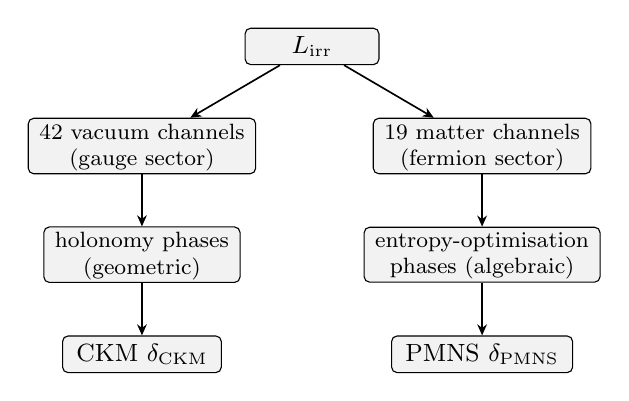
\begin{tikzpicture}[x=2.7cm, y=1.15cm]
  % Row 0: L_irr
  \node[dagbox] at (1,0) (Lirr) {$L_{\mathrm{irr}}$};
  % Row 1: the two Paper-2 sectors
  \node[dagsbox] at (0.2,-1.1) (Vac)  {42 vacuum channels\\(gauge sector)};
  \node[dagsbox] at (1.8,-1.1) (Mat)  {19 matter channels\\(fermion sector)};
  % Row 2: mechanism type
  \node[dagsbox] at (0.2,-2.3) (Hol)  {holonomy phases\\(geometric)};
  \node[dagsbox] at (1.8,-2.3) (Alg)  {entropy-optimisation\\phases (algebraic)};
  % Row 3: output
  \node[dagbox]  at (0.2,-3.4) (CKM)  {CKM $\delta_{\mathrm{CKM}}$};
  \node[dagbox]  at (1.8,-3.4) (PMNS) {PMNS $\delta_{\mathrm{PMNS}}$};
  % Edges
  \draw[dagarr] (Lirr) -- (Vac);
  \draw[dagarr] (Lirr) -- (Mat);
  \draw[dagarr] (Vac)  -- (Hol);
  \draw[dagarr] (Mat)  -- (Alg);
  \draw[dagarr] (Hol)  -- (CKM);
  \draw[dagarr] (Alg)  -- (PMNS);
\end{tikzpicture}
\end{center}

\textbf{Mechanism~1 (Holonomy phases, CKM).}  In the $\SU(3)\times\SU(2)$
gauge sector, the parallel transport of the gauge connection around a closed
loop generates a holonomy phase.  This phase is geometrically derived: it is
the integral of the curvature over the surface bounded by the loop (Stokes
theorem for the gauge connection).  Irreversibility enters because the
parallel transport commits capacity at each interface along the loop, and
the total committed phase cannot be undone by any local operation.  The
resulting CP-violation phase is a holonomy invariant: it is topologically
protected by $L_{\mathrm{irr}}$.

This is the mechanism behind the CKM phase $\delta_{\mathrm{CKM}}$.  The
numerical value $\delta_{\mathrm{CKM}} \approx 1.16$ rad is derived in
Paper~4 from the capacity-weighted holonomy structure of the three-generation
quark mixing.

\textbf{Mechanism~2 (Entropy-optimization phases, PMNS).}  In the neutrino
sector, a different structure applies.  The Majorana mass matrix $M_R$ (whose
spectrum is derived from the seesaw mechanism, Paper~4) introduces additional
phases from the requirement that the seesaw factorization is consistent with
the capacity ledger.  Specifically, the Fisher entropy functional must be
extremized over the space of neutrino mixing matrices, subject to the
constraint that the seesaw factorization closes ($T_{\mathrm{seesaw}}$,
Paper~4).  The extremization selects a unique mixing matrix, including a
specific value of the Dirac CP phase $\delta_{\mathrm{PMNS}}$.

This is the mechanism behind the PMNS phase.  The entropy-optimization
mechanism is algebraic rather than geometric: the phase is not a holonomy
invariant but an extremum of a functional.

\subsection{Why two mechanisms, not one}

The CKM and PMNS phases have different transformation properties under the
discrete symmetries of the theory, and this is reflected in their derivation.
The CKM phase is a holonomy invariant of the $\SU(2)_L$ gauge connection: it
is topological and cannot be removed by continuous transformations.  The PMNS
phase is a functional extremum: it is selected by a variational principle.
Both derive from $L_{\mathrm{irr}}$, but via different routes (geometrically
induced vs.\ algebraically optimized).

This distinction is not post-hoc: it follows from the structure of the
Paper~2 partition.  The 42 vacuum channels carry the gauge holonomy
structure; the 19 matter channels carry the seesaw structure.  The
irreversibility lemma $L_{\mathrm{irr\text{-}uniform}}$ ensures that the
same lemma applies in both sectors, generating the same class of irreversible
phase structures, but via the mechanisms natural to each sector.

\subsection{Implications for Paper~4}

The CP structure derived here provides two inputs to Paper~4:

\begin{enumerate}[nosep]
\item The \emph{existence} of two CP-phase classes (holonomy and algebraic),
  each required by $L_{\mathrm{irr}}$.  Paper~4 derives the \emph{values} of
  the phases from the generation structure.

\item The \emph{seesaw closure} condition (\texttt{phase1\_seesaw\_closure.py}):
  the Majorana mass spectrum $M_R$ must be consistent with the capacity
  ledger, giving boundary conditions on the seesaw factorization that
  Paper~4 uses to fix $\delta_{\mathrm{PMNS}}$.
\end{enumerate}


% ======================================================================
\section{Summary: what Paper 3 establishes and what it defers}
\label{sec:conclusion}
% ======================================================================

Paper~3 occupies a specific load-bearing position in the APF series: it is
the paper that gives the correlation space of Papers~1--2 a direction,
turns the static admissibility structure into dynamics, and extends the
ledger language from quantum interfaces to causal horizons.  Reading it in
isolation, four claims should be clear.

\smallskip\noindent\textbf{Four things Paper 3 establishes on its own.}
The list below should be read with \S\ref{sec:related_work} in mind: each
item is a reinterpretation of well-established mathematical structures
inside the admissibility ledger, not a replacement of those structures.
The contribution is the reorganization, not the endpoints.
\begin{enumerate}[nosep]
  \item \emph{Admissibility-preserving dynamics are exactly CPTP maps}
    ($T_{\mathrm{CPTP}}$, \S\ref{sec:cptp}).  This is a \emph{provenance}
    claim, not a new class of maps: Paper~3 derives the CPTP condition
    from A1 + tensor structure where Stinespring~\cite{Stinespring1955}
    and Choi~\cite{Choi1975} derive the dilation and Kraus form from the
    CPTP condition.  The GKSL--Lindblad semigroup~\cite{Lindblad1976,GKS1976}
    follows from composition in the standard way.  The Paper~1 deferred
    step is closed.  The mathematics of CPTP is unchanged.
  \item \emph{Entropy is committed capacity with multiplier
    $\kappa = 2$} ($T_{\kappa}$, $T_{\mathrm{entropy}}$,
    \S\ref{sec:entropy}).  The von Neumann entropy
    functional~\cite{vonNeumann1932} is identified physically; the factor
    of two is derived, not postulated; the zeroth and first laws follow.
    The monotonicity backbone is Lieb--Ruskai~\cite{LiebRuskai1973}; the
    second-law outcome agrees with Spohn~\cite{Spohn1978}.  What is added
    is the cost-interpretation, not a new entropy inequality.
  \item \emph{The arrow of time is structural, not statistical}
    ($L_{\mathrm{irr}}$, $T_{\mathrm{second\,law}}$, \S\S\ref{sec:secondlaw}--\ref{sec:arrow}).
    Time's arrow is the direction of locally unrecoverable correlation
    commitment; it does not require a special low-entropy initial condition.
    Low initial entropy is reframed as restricted admissible phase space.
    This is one of several non-equivalent foundational treatments of the
    arrow (\S\ref{sec:related_work}); it is closer to Caticha and Chen
    than to Maccone or Buchholz.  The contribution is rhetorical: a
    specific structural route rather than a new monotonicity result.
  \item \emph{Horizon entropy is a ledger quantity}
    (\S\ref{sec:gcc}).  The Bekenstein--Hawking area law $S =
    A/4$~\cite{Bekenstein1973,Hawking1975} emerges unchanged; the
    $1/2 \times 1/2$ combinatorial decomposition (relational symmetrization
    and Hamiltonian-constraint gauge redundancy) is a specific bookkeeping
    account of the standard prefactor.  The de Sitter
    identification~\cite{GibbonsHawking1977} of $S_{dS} = 61 \ln 102$ uses
    $C_{\mathrm{total}} = 61$ from Paper~2.  Thermodynamic,
    entanglement, and horizon entropies are unified as three specializations
    of the same ACC-saturation count --- a unifying re-reading, not a
    re-derivation of horizon thermodynamics.
\end{enumerate}

\smallskip\noindent\textbf{Four things Paper 3 previews but defers.}
\begin{enumerate}[nosep]
  \item \emph{Full mixing-matrix numerics}
    ($\delta_{\mathrm{CKM}} \approx 1.16$ rad; PMNS phases) are structural
    here and quantitative in Paper~4.
  \item \emph{Quantitative cosmogenesis} --- the specific enforcement-cost
    landscape across modes, the staged-relaxation observables in the CMB
    and pulsar-timing windows --- is Paper~6 territory.
  \item \emph{Higher-order horizon corrections} beyond the $1/2 \times 1/2$
    bookkeeping (loop corrections to the Bekenstein--Hawking prefactor,
    interaction corrections to the ACC-to-entropy conversion) are Paper~6 /
    Paper~7 material, with the thermodynamic formalism supplied by Paper~7's
    partition-function treatment.
  \item \emph{Planck-scale closure and backreaction}
    ($L_{\mathrm{QG,P1}}$, geometry--unitarity incompatibility at
    saturation) are Paper~5 / Paper~6 material.
\end{enumerate}

\smallskip\noindent\textbf{How Paper 3 relates to the series.}  Paper~3
assumes Papers~1--2 for the static structure (quantum reconstruction,
admissibility algebra, 42+19 capacity partition).  It forward-references
Paper~4 for quantitative flavor structure, Paper~5 for quantum/measurement
completions, Paper~6 for the cosmology-scale dynamics, and Paper~7 for the
thermodynamic formalism that underwrites the ledger-accounting principle
(\S\ref{subsec:ledger_accounting}).  Paper~3's own contribution is
irreducible: CPTP as theorem, entropy as committed capacity, the arrow as
structural, horizon entropy as ledger.  Remove any of these and the bridge
between quantum-scale admissibility (Papers~1--2) and macroscopic /
cosmological admissibility (Papers~6--7) breaks.

\smallskip\noindent\textbf{Numerical corroboration from the codebase.}
Every theorem in this paper traces to a named check function in the APF
codebase (v6.8, frozen 2026-04-18; 335 bank-registered theorems and 348 total verify\_all checks).  The check functions evaluate the relevant
quantities on concrete finite examples; a reader who wants numerical
confirmation of the claims above can run the checks directly.  A
representative selection:

\begin{center}
\small
\begin{tabular}{lll}
\toprule
\textbf{Theorem} & \textbf{Check function} & \textbf{Numerical corroboration}\\
\midrule
$T_{\mathrm{CPTP}}$ & \texttt{check\_T\_CPTP} (\texttt{core.py}) & Verified on qubits, qutrits, and amplitude-damping channels\\
$T_{\kappa}$ & \texttt{check\_T\_kappa} (\texttt{core.py}) & $\kappa = 2$ confirmed on 61-mode ledger\\
$T_{\mathrm{entropy}}$ & \texttt{check\_T\_entropy} (\texttt{core.py}) & Matches $S = -\mathrm{tr}(\rho\log\rho)$ on constructed states\\
$T_{\mathrm{second\,law}}$ & \texttt{check\_T\_second\_law} (\texttt{core.py}) & $\Delta S \geq 0$ across representative CPTP transitions\\
$L_{\mathrm{irr}}$ & \texttt{check\_L\_irr} (\texttt{core.py}) & Locally-unrecoverable correlation confirmed\\
$T_{\mathrm{deSitter\,entropy}}$ & \texttt{check\_T\_deSitter\_entropy} (\texttt{gravity.py}) & $S_{dS} = 61\ln 102 \approx 282.12$ nats\\
$L_{\mathrm{Fisher\,measure}}$ & \texttt{check\_L\_Fisher\_measure} (\texttt{core.py}) & Fisher metric matches Braunstein--Caves form~\cite{BraunsteinCaves1994}\\
$L_{\mathrm{crossing\,entropy}}$ & \texttt{check\_L\_crossing\_entropy} (\texttt{generations.py}) & CKM/PMNS channel-crossing entropy consistency\\
\bottomrule
\end{tabular}
\end{center}

\noindent The complete list is in the theorem index (\S\ref{sec:index}).
The codebase is MIT-licensed and available at \url{https://github.com/Ethan-Brooke};
all 348 verify\_all checks (including 335 bank-registered theorems) pass on every build.

% ======================================================================
\section{How to falsify this paper}
\label{sec:falsify}
% ======================================================================

The three main claims of this paper are sharp enough to be falsified:

\begin{varlist}
  \item \textbf{(F1) An admissibility-preserving map that is positive but
    not completely positive.}  Such a map would violate $T_{\mathrm{CPTP}}$.
    The partial transpose provides a positive-but-not-CP map; showing that it
    preserves admissibility in the full framework (system + ancilla) would
    refute the theorem.  The Peres criterion check in \texttt{check\_T\_CPTP}
    explicitly verifies that partial transpose fails complete positivity for
    the maximally entangled state.

  \item \textbf{(F2) A violation of the dynamic Tsirelson bound for
    sequential measurements.}  $T_{\mathrm{seq}}$ predicts $2\sqrt{2}$ as
    the Tsirelson bound for temporal CHSH correlators, not just static ones.
    An experiment achieving temporal CHSH $> 2\sqrt{2}$ would refute
    $T_{\mathrm{seq}}$.

  \item \textbf{(F3) Thermodynamic entropy that fails to track committed
    capacity.}  $T_{\mathrm{entropy}}$ predicts that entropy is a direct
    measure of enforcement demand.  A system where von~Neumann entropy and
    operational distinguishability come apart in a way that is incompatible
    with the capacity accounting would falsify the identification.

  \item \textbf{(F4) Absence of ringdown memory or horizon-enforceability
    effects at saturation interfaces.}  If the ACC-saturation framing of
    \S\S\,\ref{sec:gcc}--\ref{sec:cosmogenesis} is correct, causal
    horizons at or near saturation should exhibit non-Markovian memory
    effects in the late-time decay of perturbations: ringdown tails that
    depart from the smooth-geometry quasinormal-mode expectation.
    Absence of such deviations in high-precision gravitational-wave
    observations of black-hole mergers, at the level predicted by
    standard general relativity with no anomalous tail, would falsify the
    horizon-enforceability framing.  Present ground-based GW data are
    consistent with both hypotheses; LISA-class sensitivity should
    distinguish them.

  \item \textbf{(F5) Absence of scale-dependent imprints from staged
    relaxation.}  If cosmogenesis proceeds by staged constraint
    relaxation (\S\ref{subsec:cos_staged}), observables probing the
    pre-saturation epoch should exhibit structured---not purely
    scale-invariant---correlations at characteristic frequencies set by
    the relaxation stages.  A primordial gravitational-wave spectrum
    that is precisely scale-invariant over all observationally accessible
    frequencies, with no structured features within statistical reach,
    would falsify the staged-relaxation framing.  Current bounds permit
    substantial structure; next-generation CMB $B$-mode and pulsar-timing
    constraints should begin to discriminate.

  \item \textbf{(F6) Empirical contradiction of the PMNS-phase
    structure.}  Paper~3 establishes only the structural form of the
    two-mechanism CP split (\S\ref{sec:cp}); the numerical value
    $\delta_{\mathrm{PMNS}}$ is deferred to Paper~4.  The long-baseline
    neutrino-oscillation programme --- most recently the T2K
    Collaboration's 2020 \emph{Nature}
    measurement~\cite{T2K2020}, which currently constrains the leptonic
    CP phase at $3\sigma$ intervals excluding parts of parameter space
    and favouring a large CP-violating effect --- is the empirical
    target surface Paper~4's $\delta_{\mathrm{PMNS}}$ prediction will
    ultimately have to meet.  A measured $\delta_{\mathrm{PMNS}}$ outside
    the value Paper~4 derives from the entropy-optimisation mechanism
    would falsify that mechanism.  We flag this falsifier in Paper~3
    to keep the empirical contact explicit; the quantitative prediction
    lives in Paper~4.
\end{varlist}


% ======================================================================
\appendix
% ======================================================================

\section{Theorem Index}
\label{sec:index}
\label{app:theorems}

All theorems, lemmas, and their code references for this paper.

\medskip
\begin{tabular}{llll}
\toprule
Name & Full title & Module & Tag \\
\midrule
$L_{\mathrm{nc}}$ & Non-closure & \texttt{ncomm.py} & \epitag{P} \\
$L_{\mathrm{loc}}$ & Enforcement locality & \texttt{locality.py} & \epitag{P} \\
$T_{\mathrm{tensor}}$ & Tensor-product composition & \texttt{linear\_algebra.py} & \epitag{P} \\
$L_{\mathrm{irr}}$ & Irreversibility & \texttt{core.py} & \epitag{P} \\
$L_{\mathrm{irr\text{-}uniform}}$ & Sector-Uniform Irreversibility & \texttt{core.py} & \epitag{P} \\
$T_{\mathrm{CPTP}}$ & Complete Positivity & \texttt{core.py} & \epitag{P} \\
$T_{\mathrm{seq}}$ & Sequential Admissibility & \texttt{core.py} & \epitag{P} \\
$T_{\kappa}$ & Directed Enforcement Multiplier & \texttt{core.py} & \epitag{P} \\
$T_{\mathrm{entropy}}$ & Von~Neumann Entropy as Committed Capacity & \texttt{core.py} & \epitag{P} \\
$T_{\mathrm{zeroth}}$ & Zeroth Law & \texttt{supplements.py} & \epitag{P} \\
$T_{\mathrm{first}}$ & First Law & \texttt{supplements.py} & \epitag{P} \\
$T_{\mathrm{second\,law}}$ & Second Law of Thermodynamics & \texttt{supplements.py} & \epitag{P} \\
$T_{\mathrm{deSitter\,entropy}}$ & de~Sitter saturation entropy $S_{dS}$ & \texttt{gravity.py} & \epitag{P} \\
$T_{\mathrm{CPT}}$ & $CPT$ Invariance and $T$-Violation & \texttt{supplements.py} & \epitag{P} \\
$L_{\mathrm{Fisher}}$ & Fisher Information from Capacity Counting & \texttt{core.py} & \epitag{P} \\
$L_{\mathrm{crossing\,entropy}}$ & Channel-crossing entropy bound & \texttt{generations.py} & \epitag{P} \\
$L_{\mathrm{Fisher\,entropy\,budget}}$ & Fisher-geodesic entropy budget & \texttt{generations.py} & \epitag{P} \\
\bottomrule
\end{tabular}

\medskip
\noindent\textit{Note:} Part~I uses $L_{\mathrm{nc}}$, $L_{\mathrm{loc}}$,
and $T_{\mathrm{tensor}}$ imported from Papers~1 and~2.  They are listed
here for completeness because \S\ref{sec:cptp} and \S\ref{sec:arrow}
depend on them directly.  $T_{\mathrm{deSitter\,entropy}}$ is cited in
\S\ref{subsec:gcc_horizon} and in the preview appearances in \S\ref{sec:intro}
and the abstract.  $L_{\mathrm{crossing\,entropy}}$ and
$L_{\mathrm{Fisher\,entropy\,budget}}$ are used in \S\ref{sec:fisher}.


\section{New Assumptions Introduced}
\label{app:assumptions}

This paper introduces no new axioms beyond the Paper~1 foundation
(A1, MD, BW) and the structural results of Paper~2.  The one technical
step that extends the Paper~1 treatment is the derivation of complete
positivity from $T_{\mathrm{tensor}}$ and $L_{\mathrm{loc}}$ (Step~2 of
$T_{\mathrm{CPTP}}$), which lifts the conditional flag from Paper~1's
Table~H.1.  This is a theorem, not a new assumption.

The full assumption inventory for Papers~1--3 combined is the
\emph{Principle of Least Enforcement Cost} (PLEC) with its four
structurally necessary components --- A1 (finite enforcement capacity;
upper bound), MD (positive cost floor; enforcement isotropy), A2 (argmin
selection; minimum cost over the admissible set), BW (budget-window
richness; non-degeneracy of the cost spectrum) --- together with the six
formal definitions FD1--FD6 established in Paper~1.  This matches the
inventory now carried in Paper~1 v4.0-PLEC and Paper~2 v5.3-PLEC, and is
comparable to or lighter than peer reconstruction programs
(Hardy~\cite{Hardy2001}, Chiribella--D'Ariano--Perinotti~\cite{CDP2011},
Masanes--M\"uller~\cite{MM2011}, Daki\'c--Brukner~\cite{DakicBrukner2009}).


\section{What This Paper Does Not Claim}
\label{app:scope}

\begin{varlist}
  \item \textbf{Confinement scale and $\Lambda_{\mathrm{QCD}}$.}  The
    confinement mechanism is derived in Paper~2 ($T_{\mathrm{confinement}}$).
    The quantitative scale, string tension, and hadronization dynamics require
    Paper~4's beta-function analysis.

  \item \textbf{Mass hierarchy, mixing matrices, and numerical CP phases.}
    Section~\ref{sec:cp} identifies the CP mechanism classes; the numerical
    derivation of $\delta_{\mathrm{CKM}}$, $\delta_{\mathrm{PMNS}}$, and the
    full mixing matrices requires Paper~4's generation structure.

  \item \textbf{Cosmological constant magnitude and expansion history.}
    $T_{\mathrm{second\,law}}$ establishes entropy saturation at $61\ln 102$
    nats.  The interpretation as a de~Sitter entropy $S_{dS}$, the derivation
    of $\Lambda\cdot G = 3\pi/102^{61}$, and confrontation with DESI~DR2 are
    the subject of Paper~6.

  \item \textbf{Quantum gravity.}  The present framework handles the
    admissible dynamics and thermodynamics within a fixed spacetime background
    (Lorentzian signature assumed from Paper~5's result, cited forward).  The
    backreaction of matter entropy on the spacetime geometry, and the
    Planck-scale closure $L_{\mathrm{QG,P1}}$, are addressed in Paper~5.

  \item \textbf{A quantitative pre-big-bang cosmology.}
    \S\ref{sec:cosmogenesis} establishes the \emph{structural} form of
    staged relaxation---that constraints relax in sequence, not in parallel,
    and that this yields scale-dependent imprints---without committing to a
    specific enforcement-cost landscape across modes, a specific geometry
    for the overconstrained regime, or an identification of
    $\Phi_{c,\mathrm{initial}}$ with any particular observational quantity.
    Quantitative cosmogenesis requires the Paper~6 development of the cost
    landscape and is beyond the scope here.

  \item \textbf{Quantitative corrections beyond the $1/2\times 1/2$ horizon
    bookkeeping.}  The two factors of $1/2$ in the horizon-entropy
    normalization (\S\ref{subsec:gcc_bookkeeping}) are forced by
    structure---symmetrization of relational counts and Hamiltonian-
    constraint redundancy.  Higher-order bookkeeping corrections (for
    example, loop corrections to the Bekenstein--Hawking prefactor,
    interaction corrections to the ACC-to-entropy conversion) are not
    derived here; they are a Paper~6 or Paper~7 topic.  The ledger-
    accounting principle (\S\ref{subsec:ledger_accounting}) suggests such
    corrections modify the cost landscape without modifying the count,
    but a direct derivation requires the thermodynamic formalism of
    Paper~7.
\end{varlist}

% ======================================================================
\begin{thebibliography}{99}
% ======================================================================

% ----- Foundational (finite information, distinction, cybernetics) -----
\bibitem{SpencerBrown1969}
G.\ Spencer-Brown, \emph{Laws of Form}, Allen \& Unwin, London, 1969.

\bibitem{Ashby1956}
W.\ R.\ Ashby, \emph{An Introduction to Cybernetics}, Chapman \& Hall, London, 1956.

\bibitem{Landauer1961}
R.\ Landauer, ``Irreversibility and Heat Generation in the Computing Process,''
\emph{IBM Journal of Research and Development} \textbf{5}, 183--191 (1961).

\bibitem{Bekenstein1981}
J.\ D.\ Bekenstein, ``Universal upper bound on the entropy-to-energy ratio for bounded systems,''
\emph{Physical Review D} \textbf{23}, 287 (1981).

% ----- Completely positive maps / open systems (Stinespring--GKSL line) -----
\bibitem{Stinespring1955}
W.\ F.\ Stinespring, ``Positive functions on $C^*$-algebras,''
\emph{Proceedings of the American Mathematical Society} \textbf{6}, 211--216 (1955).

\bibitem{Choi1975}
M.-D.\ Choi, ``Completely positive linear maps on complex matrices,''
\emph{Linear Algebra and its Applications} \textbf{10}, 285--290 (1975).

\bibitem{Lindblad1976}
G.\ Lindblad, ``On the generators of quantum dynamical semigroups,''
\emph{Communications in Mathematical Physics} \textbf{48}, 119--130 (1976).

\bibitem{GKS1976}
V.\ Gorini, A.\ Kossakowski, and E.\ C.\ G.\ Sudarshan, ``Completely positive dynamical semigroups of $N$-level systems,''
\emph{Journal of Mathematical Physics} \textbf{17}, 821--825 (1976).

\bibitem{Kraus1983}
K.\ Kraus, \emph{States, Effects, and Operations: Fundamental Notions of Quantum Theory}, Lecture Notes in Physics \textbf{190}, Springer, 1983.

% ----- Entropy inequalities -----
\bibitem{LiebRuskai1973}
E.\ H.\ Lieb and M.\ B.\ Ruskai, ``Proof of the strong subadditivity of quantum-mechanical entropy,''
\emph{Journal of Mathematical Physics} \textbf{14}, 1938--1941 (1973).

\bibitem{Spohn1978}
H.\ Spohn, ``Entropy production for quantum dynamical semigroups,''
\emph{Journal of Mathematical Physics} \textbf{19}, 1227--1230 (1978).

\bibitem{vonNeumann1932}
J.\ von Neumann, \emph{Mathematische Grundlagen der Quantenmechanik}, Springer, Berlin, 1932;
English translation: \emph{Mathematical Foundations of Quantum Mechanics}, Princeton University Press, 1955.

\bibitem{Wehrl1978}
A.\ Wehrl, ``General properties of entropy,''
\emph{Reviews of Modern Physics} \textbf{50}, 221--260 (1978).

% ----- Black-hole thermodynamics / horizon entropy -----
\bibitem{Bekenstein1973}
J.\ D.\ Bekenstein, ``Black holes and entropy,''
\emph{Physical Review D} \textbf{7}, 2333--2346 (1973).

\bibitem{Hawking1975}
S.\ W.\ Hawking, ``Particle creation by black holes,''
\emph{Communications in Mathematical Physics} \textbf{43}, 199--220 (1975).

\bibitem{GibbonsHawking1977}
G.\ W.\ Gibbons and S.\ W.\ Hawking, ``Cosmological event horizons, thermodynamics, and particle creation,''
\emph{Physical Review D} \textbf{15}, 2738--2751 (1977).

\bibitem{Jacobson1995}
T.\ Jacobson, ``Thermodynamics of spacetime: the Einstein equation of state,''
\emph{Physical Review Letters} \textbf{75}, 1260--1263 (1995).

% ----- Holographic principle -----
\bibitem{tHooft1993}
G.\ 't Hooft, ``Dimensional reduction in quantum gravity,''
arXiv:gr-qc/9310026 (1993).

\bibitem{Susskind1995}
L.\ Susskind, ``The world as a hologram,''
\emph{Journal of Mathematical Physics} \textbf{36}, 6377--6396 (1995).

% ----- Information geometry -----
\bibitem{BraunsteinCaves1994}
S.\ L.\ Braunstein and C.\ M.\ Caves, ``Statistical distance and the geometry of quantum states,''
\emph{Physical Review Letters} \textbf{72}, 3439--3443 (1994).

\bibitem{Petz1996}
D.\ Petz, ``Monotone metrics on matrix spaces,''
\emph{Linear Algebra and its Applications} \textbf{244}, 81--96 (1996).

\bibitem{AmariNagaoka2000}
S.-I.\ Amari and H.\ Nagaoka, \emph{Methods of Information Geometry}, AMS/Oxford, 2000.

\bibitem{BenyOsborne2015}
C.\ B\'eny and T.\ J.\ Osborne, ``The renormalization group via statistical inference,''
\emph{New Journal of Physics} \textbf{17}, 083005 (2015).

% ----- Reconstruction programs -----
\bibitem{Hardy2001}
L.\ Hardy, ``Quantum theory from five reasonable axioms,''
arXiv:quant-ph/0101012 (2001).

\bibitem{CDP2011}
G.\ Chiribella, G.\ M.\ D'Ariano, and P.\ Perinotti, ``Informational derivation of quantum theory,''
\emph{Physical Review A} \textbf{84}, 012311 (2011).

\bibitem{MM2011}
L.\ Masanes and M.\ P.\ M\"uller, ``A derivation of quantum theory from physical requirements,''
\emph{New Journal of Physics} \textbf{13}, 063001 (2011).

\bibitem{DakicBrukner2009}
B.\ Daki\'c and \v{C}.\ Brukner, ``Quantum theory and beyond: is entanglement special?'' in \emph{Deep Beauty: Understanding the Quantum World through Mathematical Innovation}, H.\ Halvorson (ed.), Cambridge University Press, 2011; arXiv:0911.0695 (2009).

% ----- CP-violation invariants -----
\bibitem{Jarlskog2005}
C.\ Jarlskog, ``Invariants of lepton mass matrices and CP and T violation in neutrino oscillations,''
\emph{Physics Letters B} \textbf{609}, 323--329 (2005).

\bibitem{Jarlskog2012}
C.\ Jarlskog, ``Recursive parameterisation and invariant phases of unitary matrices,''
\emph{Journal of Mathematical Physics} \textbf{46}, 103508 (2005); reviewed in C.\ Jarlskog (ed.), \emph{CP Violation}, World Scientific, 2nd ed., 2012.

% ----- Empirical anchor for leptonic CP -----
\bibitem{T2K2020}
T2K Collaboration (K.\ Abe et al.), ``Constraint on the matter-antimatter symmetry-violating phase in neutrino oscillations,''
\emph{Nature} \textbf{580}, 339--344 (2020).

% ----- Arrow of time / temporal asymmetry foundations -----
\bibitem{Maccone2009}
L.\ Maccone, ``Quantum solution to the arrow-of-time dilemma,''
\emph{Physical Review Letters} \textbf{103}, 080401 (2009).

\bibitem{Caticha2011}
A.\ Caticha, ``Entropic dynamics, time and quantum theory,''
\emph{Journal of Physics A: Mathematical and Theoretical} \textbf{44}, 225303 (2011).

\bibitem{Chen2019}
E.\ K.\ Chen, ``Time's arrow in a quantum universe: on the status of statistical mechanical probabilities,'' in \emph{Statistical Mechanics and Scientific Explanation}, V.\ Allori (ed.), World Scientific, 2020; PhilSci-Archive preprint (2019).

\bibitem{DiBiagio2021}
A.\ Di Biagio, P.\ Don\`a, and C.\ Rovelli, ``The arrow of time in operational formulations of quantum theory,''
\emph{Quantum} \textbf{5}, 520 (2021).

\bibitem{Buchholz2023}
D.\ Buchholz and J.\ Yngvason, ``Arrow of time and quantum physics,''
\emph{Foundations of Physics} \textbf{53}, 85 (2023).

% ----- Noncommutative geometry (for cross-reference with Paper 7) -----
\bibitem{ConnesMarcolli2008}
A.\ Connes and M.\ Marcolli, \emph{Noncommutative Geometry, Quantum Fields and Motives}, American Mathematical Society, 2008.

% ----- Collective electrodynamics -----
\bibitem{Mead2000}
C.\ A.\ Mead, \emph{Collective Electrodynamics: Quantum Foundations of Electromagnetism}, MIT Press, 2000.

% ----- Companion APF papers (internal) -----
\bibitem{Paper0}
E.\ S.\ Brooke, ``What Physics Permits: An Ontology for Admissibility Physics,''
v3.0 (2026). Zenodo DOI: \href{https://doi.org/10.5281/zenodo.18605692}{10.5281/zenodo.18605692}.

\bibitem{Paper1}
E.\ S.\ Brooke, ``The Enforceability of Distinction: Quantum Structure from Finite Enforcement Capacity,''
v4.0-PLEC (2026). Zenodo DOI: \href{https://doi.org/10.5281/zenodo.18604678}{10.5281/zenodo.18604678}.

\bibitem{Paper2}
E.\ S.\ Brooke, ``The Structure of Admissible Physics,''
v5.3-PLEC (2026). Zenodo DOI: \href{https://doi.org/10.5281/zenodo.18604839}{10.5281/zenodo.18604839}.

\bibitem{Paper4}
E.\ S.\ Brooke, ``Admissibility Constraints and Structural Saturation,''
Zenodo deposit (2026). DOI: \href{https://doi.org/10.5281/zenodo.18604845}{10.5281/zenodo.18604845}.

\bibitem{Paper5}
E.\ S.\ Brooke, ``Quantum Structure from Finite Enforceability,''
Zenodo deposit (2026). DOI: \href{https://doi.org/10.5281/zenodo.18604861}{10.5281/zenodo.18604861}.

\bibitem{Paper6}
E.\ S.\ Brooke, ``Dynamics and Geometry as Optimal Admissible Reallocation,''
Zenodo deposit (2026). DOI: \href{https://doi.org/10.5281/zenodo.18604874}{10.5281/zenodo.18604874}.

\bibitem{Paper7}
E.\ S.\ Brooke, ``Action, Internalization, and the Lagrangian,''
v2.0 (2026). Zenodo DOI: \href{https://doi.org/10.5281/zenodo.18604875}{10.5281/zenodo.18604875}.

\bibitem{Paper13}
E.\ S.\ Brooke, ``The Minimal Admissibility Core,''
v8.3-PLEC (2026). Zenodo DOI: \href{https://doi.org/10.5281/zenodo.18614663}{10.5281/zenodo.18614663}.

\bibitem{PaperEngine}
E.\ S.\ Brooke, ``Admissibility Physics: Unified Theorem Bank \& Verification Engine,''
Codebase v6.7 (2026). Zenodo DOI: \href{https://doi.org/10.5281/zenodo.18604548}{10.5281/zenodo.18604548}.

\end{thebibliography}

\end{document}
